\documentclass[a4paper,12pt,headsepline]{report}

%----------------- PDF CONFIG ----------------- %
\pdfinfo{    
     /Title (Permissioned Blockchains für B2B - Prototypische Implementierung eines dezentralisierten Wartungsmarktes) 
     /Subject   (Permissioned Blockchains)    
     /Author  (Eric Nagel) 
     /Keywords   (Blockchain, B2B)      
}

\title{Permissioned Blockchains für B2B - Prototypische Implementierung eines dezentralisierten Wartungsmarktes}
\author{Eric Nagel}
\date{09.03.2018}



%----------------- PAKETE INKLUDIEREN ----------------- %

\usepackage{geometry} % Packet für Seitenrandabständex und Einstellung für Seitenränder
\usepackage[ngerman]{babel} % deutsche Silbentrennung

\usepackage{booktabs} %entzerrt die Tabellenzeilen und bietet verschieden dicke Unterteilungslinien
\usepackage{longtable} % Tabellen können sich nicht über mehrere Seiten 
\usepackage{graphicx} % kann LaTeX Grafiken einbinden

\usepackage[utf8]{inputenc}
\usepackage[T1]{fontenc} % Zeichenencoding
\usepackage{lmodern} % typographische Qualität 
\frenchspacing % Schaltet den zusätzlichen Zwischenraum ab
\usepackage{fix-cm}
\usepackage{hyperref} % verwandelt alle Kapitelüberschriften, Verweise aufs Literaturverzeichnis und andere Querverweise in PDF-Hyperlinks
\usepackage{color}
\usepackage{url}
\usepackage{enumitem}
\setitemize{itemsep=-5pt}

\usepackage[nottoc]{tocbibind}

% für Listings
\usepackage{listings}
\lstset{numbers=left, numberstyle=\tiny, numbersep=5pt, stepnumber=4, keywordstyle=\color{black}\bfseries\itshape, stringstyle=\ttfamily,showstringspaces=false,basicstyle=\footnotesize,captionpos=b}
\lstset{language=java}

%----------------- FARBEN DEFINIEREN ----------------- %
\definecolor{gray}{gray}{0.95} % Listingsbackground

%----------------- LAYOUT SETZEN ----------------- %
\geometry{left=2cm, right=2cm, top=2.5cm, bottom=2cm}
\linespread {1.25}\selectfont %1.25 da er von Haus aus 1.2 ist und 1,25 * 1,2 = 1,5 isch

%%----------------- INHALT -----------------%

%TODO: Datum für Webartikel etc. in Zotero einfügen
%TODO: Spellcheck
%TODO: Proofreading
\begin{document}

\pagenumbering{roman} % Seitennummer

 %----------------- KONFIGURATION ----------------- %
\pagestyle{empty} % enthalten keinerlei Kopf oder Fuß 

%----------------- HDA FBI Logo ----------------- %
\begin{figure}[t]
	\centering
	
\includegraphics[width=0.6\textwidth]{images/logo_fbi}
\end{figure}

%----------------- INHALT ----------------- %

\begin{center}
\Large Hochschule Darmstadt \\
\normalsize \textsc{- Fachbereich Informatik -} \\

% Whitespace
\vspace{80 pt}

\Huge Permissioned Blockchains für B2B \\ 
\Large Prototypische Implementierung eines dezentralisierten Wartungsmarktes \\
\normalsize
\vspace{20 pt}

Abschlussarbeit zur Erlangung des akademischen Grades \\ 
Bachelor of Science (B.Sc.) 

\vspace{75 pt}


vorgelegt von \\
\vspace{5 pt}
Eric Nagel \\
Matrikelnummer 740693
\vspace{80 pt}

\begin{tabular}[h]{p{4cm}l l}
	Referent: & Prof. Dr. Andreas Müller \\
	Korreferent: & Björn Bär
\end{tabular}


\end{center}


 %----------------- KONFIGURATION ----------------- %
\pagestyle{empty} % enthalten keinerlei Kopf oder Fuß

%TODO: Abstract eventuell auf 3/4 Seite verlängern
\chapter*{Zusammenfassung} % (fold)
\addcontentsline{toc}{chapter}{Zusammenfassung}
\label{cha:abtract}

Traditionelle B2B-Anwendungen, mit multiplen Unternehmen als Teilnehmer, bringen Probleme bezüglich der Datenhaltung mit sich. Eine Option ist, dass jedes Unternehmen Daten bei sich selber speichert. Dies führt jedoch zu zusätzlichen Aufwand, da Schnittstellen eingerichtet werden müssen, um Geschäftspartnern Zugriff auf relevante Daten zu gewähren. Eine weitere Option ist die Speicherung bei einer zentralen, verwaltenden Instanz. Jeder Geschäftspartner müsste dieser jedoch vertrauen, was die Anwendung unattraktiver macht. Eine Lösung für diese Probleme könnte die Blockchain-Technologie darstellen. Mit ihr ist eine verteilte Datenspeicherung unter nicht vertrauenswürdigen Teilnehmern möglich. Dabei stellt die Blockchain sicher, dass die Daten bei allen Geschäftspartnern synchron sind, und nicht manipuliert oder gelöscht werden können. Die Technologie bringt jedoch auch Schwierigkeiten mit sich, welche für B2B-Anwendungen unerwünscht sind. In Public Blockchains wie Bitcoin und Ethereum äußert sich dies anhand der Skalierbarkeit, Performance und Sicherheit. Permissioned Blockchains, wie Hyperledger Fabric, können diese Probleme zu Teilen lösen. Nichtsdestotrotz sind darauf basierende Anwendungen auf eine bestimmte Performance oder Nutzerzahl limitiert. Auf Grundlage dieser Erkenntnisse wurde ein Prototyp eines automatisierten dezentralen Wartungsmarktes als Proof-of-Concept entwickelt. In diesen können IoT-Geräte Wartungsbedarf erkennen und Wartungsanbieter darauf reagieren.

 
\tableofcontents % Inhaltverzeichnis

\listoffigures % Abbildungen

\listoftables % Tabellen

\renewcommand{\lstlistlistingname}{Listingverzeichnis}
\lstlistoflistings

\pagestyle{plain} % zurueck setzen von roemische seitenanzahl

\pagenumbering{arabic}
\chapter{Einführung und Motivation}
\label{cha:einfuehrung}

Klassische \acs{B2B}-Anwendungen bringen Probleme hinsichtlich der Datenhaltung mit sich. Eine Option ist die Speicherung der Daten jeden Geschäftspartner selbst. Der Datenzugriff untereinander ist dann jedoch, aufgrund von aufwendig einzurichtenden Schnittstellen und uneinheitlichen Datenformaten, erschwert. Eine weitere Möglichkeit ist die Speicherung bei einem zentralen Unternehmen. Dieses hätte jedoch die Kontrolle über die Daten, womit alle anderen Parteien diesem vertrauen müssten. Diese Faktoren machen \acs{B2B}-Anwendungen für die Teilnehmer unattraktiv und erschweren die Entwicklung \cite{KorpelaDigitalSupplyChain2017}\cite{WustyouneedBlockchain2017}.

Um diese Probleme zu lösen, wird ein Prototyp einer dezentralen \acs{B2B}-Applikation, basierend auf der Blockchain-Technologie, entwickelt. Sie erlaubt es, dezentrale Systeme aufzubauen, in welchen sich die Parteien nicht vertrauen. Alle Daten würden bei jedem Teilnehmer des Blockchain-Netzwerks (im Folgenden nur noch Netzwerk genannt) gespeichert werden. Trotzdem sind diese nicht lösch- oder manipulierbar, alle Transaktionen sind lückenlos nachvollziehbar und es besteht ein gemeinsamer Konsens über den Datenbestand \cite{CrosbyBlockChainTechnologyBitcoin2016}.

Bekannte Blockchain-Implementationen, wie Bitcoin oder Ethereum, bringen jedoch Probleme für den \acs{B2B}-Bereich mit sich. So sind alle Daten öffentlich einsehbar, der Transaktionsdurchsatz ist gering und die Konsensmechanismen sind unter bestimmten Umständen unsicher und resultieren in hohen Energieverbrauch \cite{Gramolidangerprivateblockchains2016}\cite{NakamotoBitcoinPeertoPeerElectronic2008}\cite{EthereumTeamEthereumWhitePaper2017}. 

Ziel dieser Arbeit ist es, die Probleme der Blockchain-Technologie für den \acs{B2B}-Bereich zu analysieren und basierend auf den Ergebnissen eine dezentrale \acs{B2B}-Anwendung als Proof-of-Concept zu entwickeln. Dazu werden zunächst die grundlegenden Konzepte der Blockchain-Technologie erläutert, um ein besseres Verständnis für die Vor- und Nachteile dieser zu erhalten. Anschließend werden die Probleme für \acs{B2B}-Anwendungen anhand der Anforderungen an diese genauer betrachtet und analysiert. Daraufhin erfolgt die Beschreibung der Anwendungsentwicklung. Zuletzt wird ein Fazit zur Lösung der Probleme und des entwickelten Systems gezogen.

\chapter{Grundlagen}
\label{cha:grundlagen}
Zum Verstehen der Diskussion der Probleme der Blockchain-Technologie ist es notwendig, die grundlegenden Konzepte dieser zu verstehen. Weiterhin müssen allgemeine Anforderungen an B2B-Anwendungen erfasst werden, anhand welchen die Diskussion erfolgt.

\section{Blockchain}

\subsection{Funktionsweise}
Die Funktionsweise der Blockchain wird in dieser Arbeit hauptsächlich am Beispiel von Bitcoin erklärt. Als erste Blockchain-Anwendung \cite{ZhengBlockchainChallengesOpportunities2017} und aufgrund der überschaubaren Komplexität liefert es die Grundlage für die Funktionsweise der Technologie. Andere Implementationen, wie Ethereum oder Ripple, funktionieren nach dem gleichen Prinzip.

\subsubsection{Allgemein}
Wenn der Begriff ``Die Blockchain'' auftaucht, ist damit meistens die Blockchain-Technologie gemeint. Es gibt nicht nur eine global bestehende Blockchain und auch nicht nur eine Implementation der Technologie, was beispielsweise anhand von Bitcoin und Ethereum ersichtlich ist.

Allgemein kann die Blockchain als Datenstruktur bezeichnet werden, welche verteilt, nicht lösch- und manipulierbar gespeichert werden kann. Weiterhin verifizieren jegliche Teilnehmer am Netzwerk ausgeführte Transaktionen, wodurch ein gemeinsamer Konsens über den Datenbestand besteht \cite{CrosbyBlockChainTechnologyBitcoin2016}.

In einer Blockchain werden Transaktionen in Blöcken gespeichert. Dabei handelt es sich um Operationen, welche Daten erstellen und manipulieren. Aus diesen lässt sich letztendlich der aktuelle Datenbestand ermitteln. So erfolgt beispielsweise bei Bitcoin keine Speicherung des aktuellen Guthabens der Teilnehmer. Es wird nur aus allen bestehenden Transaktionen berechnet \cite[S.~85]{AntonopoulosMasteringbitcoin2015}. Die Daten, welche letztendlich bestehen, können beispielsweise Geldtransferinformationen (Bitcoin), Smart Contracts (Ethereum, selbst ausführende Verträge mit selbst erstellter Programmlogik, siehe \ref{subsec:use-cases}), simple Dokumente oder Informationen sein \cite{EthereumTeamEthereumWhitePaper2017}\cite{NakamotoBitcoinPeertoPeerElectronic2008}\cite{HyperledgerFabricTeamHyperledgerWhitepaper2016}. Die Blöcke setzen sich aus den Transaktionen sowie den Block Header zusammen, welcher verschiedene Metadaten, wie zum Beispiel den kombinierten Hash\footnote{Hash: Ergebnis einer Operation, welche Daten in eine Zeichenfolge fester Länge umwandelt \cite[S.~\Rn{7}]{SwanBlockchainblueprintnew2015}.} aller Transaktionen, enthält \cite[S.~160-161]{AntonopoulosMasteringbitcoin2015}.

Die Blöcke sind miteinander verkettet. Jeder Block Header enthält den Hash  des vorherigen Block Headers (siehe Abb. \ref{fig:block-chain}). Dies ist ein wichtiges Feature zum Schutz der Blockchain vor Angriffen. Wenn ein Angreifer die Transaktionen eines Blocks zu seinen Gunsten verändern würde, würde sich der Hash des Block Headers ändern. Dieser müsste dann im darauffolgenden Block Header stehen, wodurch sich allerdings auch der Hash dieses Blocks ändert. Letztendlich müssten alle nachfolgenden Blöcke manipuliert werden, um eine gültige Blockchain zu erhalten \cite{NakamotoBitcoinPeertoPeerElectronic2008}. Diese Manipulation wird durch verschiedene Verfahren erschwert, welche genauer in den Kapiteln \ref{subsec:konsens} und \ref{subsec:immutability} erklärt werden.

\begin{figure}[!htbp]
  \centering
	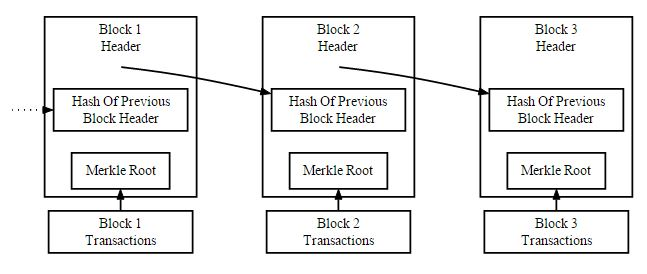
\includegraphics[width=0.85\textwidth,angle=0]{images/block-chain}
 	\caption{Verkettung von Blöcken durch Block Header Hashes \cite{RosicWhatHashingHood2017}.}
	\label{fig:block-chain}
\end{figure}

Die Blockchain ist verteilt gespeichert. Jeder Teilnehmer hat die Möglichkeit Sie auf seinen Rechner zu speichern. Somit besteht keine zentrale Instanz, welche die Kontrolle über die Daten hat. Weiterhin gibt es keinen Single Point of Failure\footnote{Single Point of Failure: Komponente eines Systems, dessen Ausfall den Ausfall des gesamten Systems bewirkt \cite{KshetriCanBlockchainStrengthen2017}.} \cite{KshetriCanBlockchainStrengthen2017}.

\label{subsec:konsens}
\subsubsection{Konsensmechanismen}
Aufgrund der verteilten Datenhaltung muss es Verfahren geben, um die Daten synchron und auf einen Stand, auf welchen sich alle Teilnehmer geeinigt haben, zu halten. Dazu gibt es die sogenannten Konsensmechanismen, welche gleichzeitig die Manipulierbarkeit der Daten verhindern. Bevor diese erklärt werden können, muss zunächst genauer auf die Funktion des Netzwerks eingegangen werden.

\paragraph{Funktion des Netzwerks}
Wenn ein Teilnehmer eine Transaktion ausführt, wird diese, vorausgesetzt dass sie valide ist (genauer im nächsten Absatz erklärt), an alle Nodes\footnote{Node: Teilnehmer eines Blockchain-Netzwerks, welche die Blockchain speichern. Auch Peers genannt.} im Netzwerk weitergeleitet und im Transaktionspool aufgenommen. Dieser enthält alle noch nicht in Blöcken vorkommenden Transaktionen. Diese werden in einen neuen Block aufgenommen, während jede Node mit der Erstellung von diesem beschäftigt ist. Dies wird durch verschiedene Konsensmechanismen realisiert. Bei Bitcoin und Ethereum findet der \acl{PoW} (\acs{PoW}) Anwendung (weiter unten genauer unter erklärt). Sobald eine Node einen Block erstellt, wird dieser im Netzwerk verteilt. Jede Node hängt ihn an ihre lokale Blockchain an und beginnt mit der Erstellung des nächsten Blocks \cite[S.~200 ff.]{AntonopoulosMasteringbitcoin2015}.

Damit eine Transaktion valide ist, muss sie bestimmte Voraussetzungen erfüllen. So muss sie unter anderem mit dem Private Key des Senders signiert sein. Mittels seines Public Keys kann überprüft werden, ob wirklich er der Sender der Nachricht ist und ob die Transaktion manipuliert wurde. Dieses Verfahren wird auch in der Abbildung \ref{fig:key-signing} visualisiert. Das Signieren trägt zur Sicherheit der Blockchain bei, da ein Angreifer dadurch keine Transaktionen eines Nutzers manipulieren oder in seinem Namen ausführen kann. In Bitcoin ist eine weitere Kondition, dass der Transaktionsersteller die zu sendenden Bitcoins besitzt \cite[S.~18]{AntonopoulosMasteringbitcoin2015}. In Systemen wie Ethereum und Hyperledger Fabric, in welchen eigene Programmlogik abgebildet werden kann, können weitere Konditionen festgelegt werden. So muss beispielsweise ein Teilnehmer die nötigen Rechte haben um eine Transaktion auszuführen (siehe \ref{acl}) \cite{HyperledgerComposerTeamAccessControlLanguage}.

\begin{figure}[!htbp]
	\centering
	  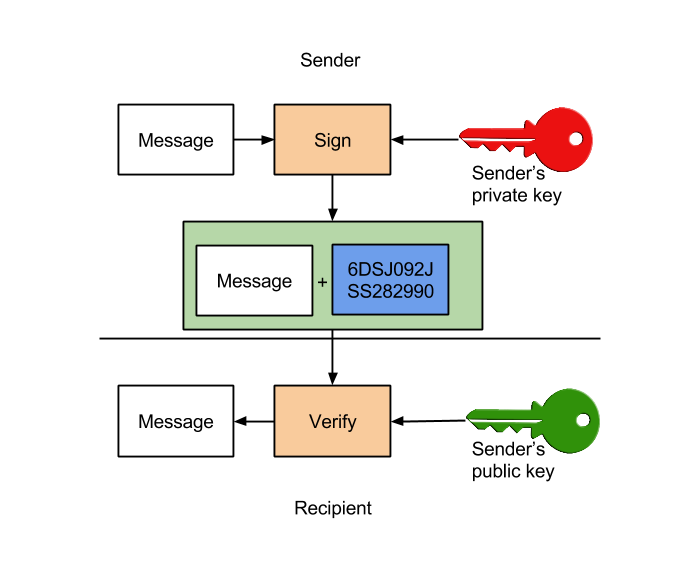
\includegraphics[width=0.4\textwidth,angle=0]{images/key-signing}
	  \caption{Signieren und Verifizieren von Nachrichten. Der Sender signiert die Nachricht mit seinem Private Key und der Empfänger kann diese mit den Public Key des Senders verifizieren \cite{WikimediaCommonsPublickeysigning2006}.}
	  \label{fig:key-signing}
\end{figure}
	
\paragraph{Proof-of-Work}
Der \acs{PoW} ist nur einer der zur Verfügung stehenden Konsensmechanismen (siehe Kapitel \ref{sec:eval-konsens}). Er bedarf jedoch genauerer Erklärung, da er in aktuellen Blockchain-Implementationen vorwiegend genutzt wird. Der \acs{PoW} ist eine Art Rätsel, welches mit der Rechenleistung von Nodes gelöst werden muss, um einen Block zu erschaffen (das sogenannte \textit{Mining}). Genauer gesagt, muss für einen Block ein Hash gefunden werden, welcher einen bestimmten Wert unterschreitet. Um unterschiedliche Hashwerte für gleich bleibende Blöcke zu erhalten, gibt es im Block Header eine Nonce\footnote{Nonce: Eine Nummer, welche genau einmal für einen bestimmten Zweck genutzt wird \cite{MargaretNonceDefinition}.}, welche verändert wird \cite{NakamotoBitcoinPeertoPeerElectronic2008}. Alle Nodes im Netzwerk ändern diese so lange, bis ein gültiger Hash gefunden wird. Desto kleiner der zu findende Hash ist, desto höher ist die Schwierigkeit. Für Sicherheitszwecke ist es nötig, dass die Blockerstellung eine gewisse Zeit benötigt. Um wachsender Rechenleistung und Teilnehmerzahl entgegenzuwirken und somit diese Zeit zu garantieren, kann die Schwierigkeit angepasst werden. Dies wird genauer im Kapitel \ref{sec:scalability-eval} erläutert. Damit die Nodes eine Motivation haben, Rechenleistung für das Erstellen von Blöcken zu nutzen, erhalten sie bei Erbringung des \acs{PoW} eine Belohnung sowie die Transaktionsgebühren in Form von Kryptowährung. In Verbindung mit den Mining sind auch Mining Pools zu erwähnen. Dabei handelt es sich um einen Zusammenschluss von Minern, welche gemeinsam probieren den \acs{PoW} zu erbringen. Gelingt dies, wird die Belohnung zwischen allen Teilnehmern im Pool geteilt.  \cite{NakamotoBitcoinPeertoPeerElectronic2008} \cite{EthereumTeamEthereumWhitePaper2017}. 

\paragraph{Forking}
Um vollständig zu verstehen, wie der \acs{PoW} funktioniert, muss das Forking erklärt werden. Wenn eine Node einen \acs{PoW} erbringt, also einen Block erstellt, wird dieser an alle anderen Nodes weitergeleitet. Im Bitcoin-Netzwerk dauert es bei einer maximalen Blockgröße von 1 MB \cite{SchererPerformanceScalabilityBlockchain2017}, zwischen 6 und 20 Sekunden, bis ein Block mindestens 90 \% aller Nodes erreicht hat \cite{BitcoinStatsBitcoinPropagationData}. Dies stimmt auch mit dem Paper von Decker und Wattenhofer überein, wo eine durchschnittliche Zeit von 12,6 Sekunden angegeben wird, bis ein Block 95 \% aller Nodes erreicht \cite{DeckerInformationpropagationbitcoin2013}. In dieser Zeit kann es vorkommen, dass eine weitere Node einen Block erstellt. Auch dieser wird im Netzwerk verteilt, wodurch zwei Versionen der Blockchain existieren: Eine endet mit Block A und die andere mit Block B. Dies ist der sogenannte Fork. Das Netzwerk muss sich nun darauf einigen, welche der beiden Versionen beibehalten werden soll. Deshalb gilt: Die Blockchain, in welche mehr Arbeit eingeflossen ist, ist die gültige. Im Falle von Bitcoin wäre dies die längere Blockchain. Die Nodes probieren an den zuerst erhaltenen Block (A oder B) einen neuen anzuhängen. Gelingt dies, ist eine der beiden Blockchains länger als die andere. Diese wird dann von allen Nodes als die richtige akzeptiert. Dieser Vorgang wird auch in den Abbildungen \ref{fig:fork_1} bis \ref{fig:fork_4} dargestellt. Theoretisch ist es möglich, dass ein Fork über mehrere Blöcke besteht. Die Wahrscheinlichkeit dafür ist jedoch gering, da mehrmals nacheinander mindestens zwei Nodes zur ungefähr gleichen Zeit einen Block erstellen müssen. Auch zu erwähnen ist, dass in einem Fork-Branch weitere Forks entstehen können. Diese Forks sind der Grund, warum Transaktionen erst als bestätigt gelten, sobald sie in einem Block stehen, welcher eine gewisse Anzahl an Nachfolgern hat. Denn erst dann ist die Sicherheit gegeben, dass die Transaktion nicht in einem Branch vorhanden ist, welcher eventuell verworfen wird \cite[S.~211 ff.]{AntonopoulosMasteringbitcoin2015}. Wie genau der \acs{PoW} das Netzwerk absichert, wird im Kapitel \ref{subsec:immutability} erklärt.

\begin{figure}[!htbp]
  \centering
    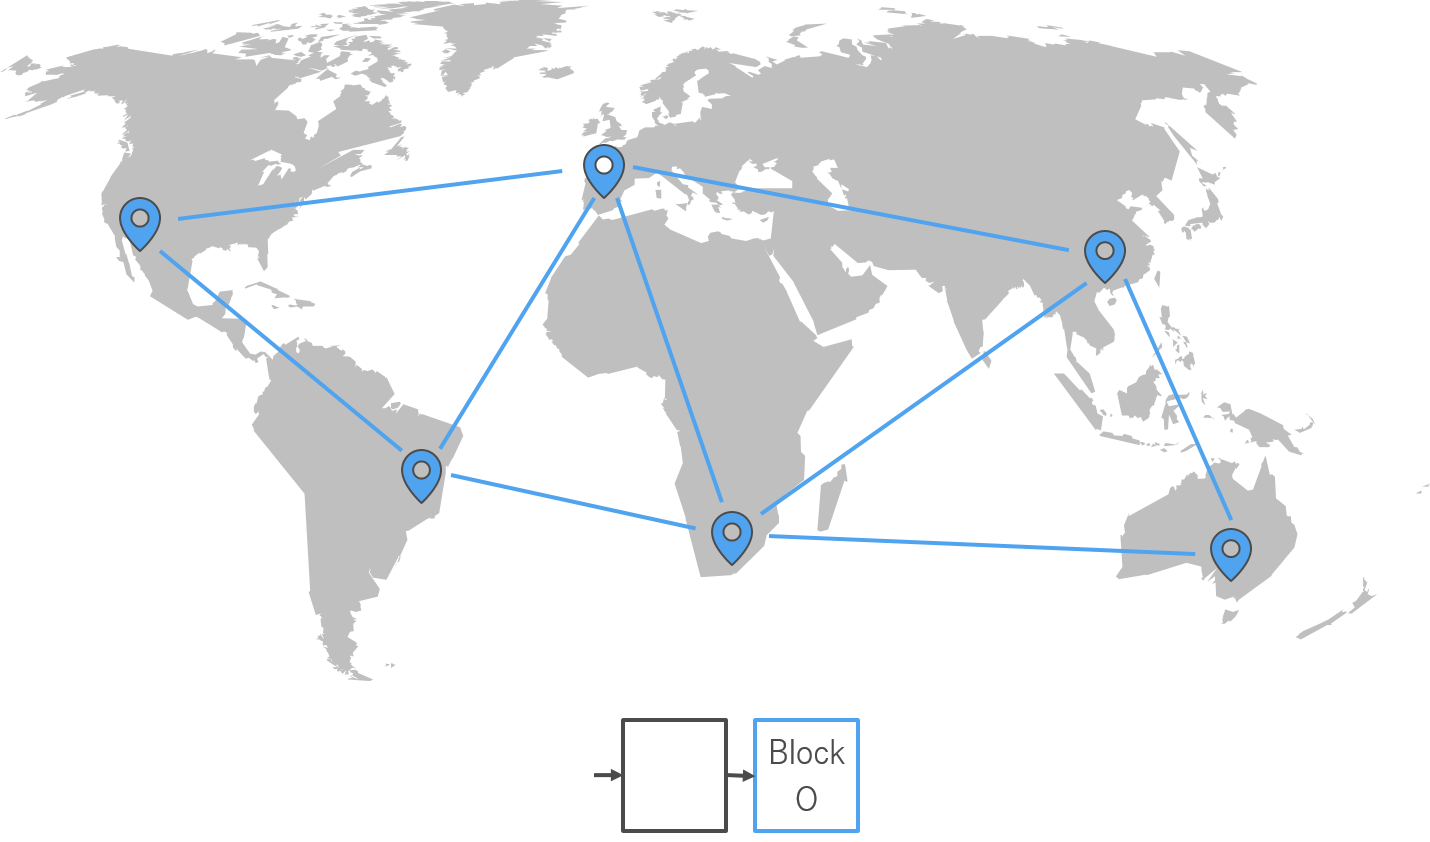
\includegraphics[width=0.95\textwidth,angle=0]{images/fork_1}
 	\caption{Fork-Visualisierung - Vor dem Fork besitzen alle Nodes Block O als letzten Block \cite[S.~200 ff.]{AntonopoulosMasteringbitcoin2015}.}
	\label{fig:fork_1}
\end{figure}

\begin{figure}[!htbp]
  \centering
	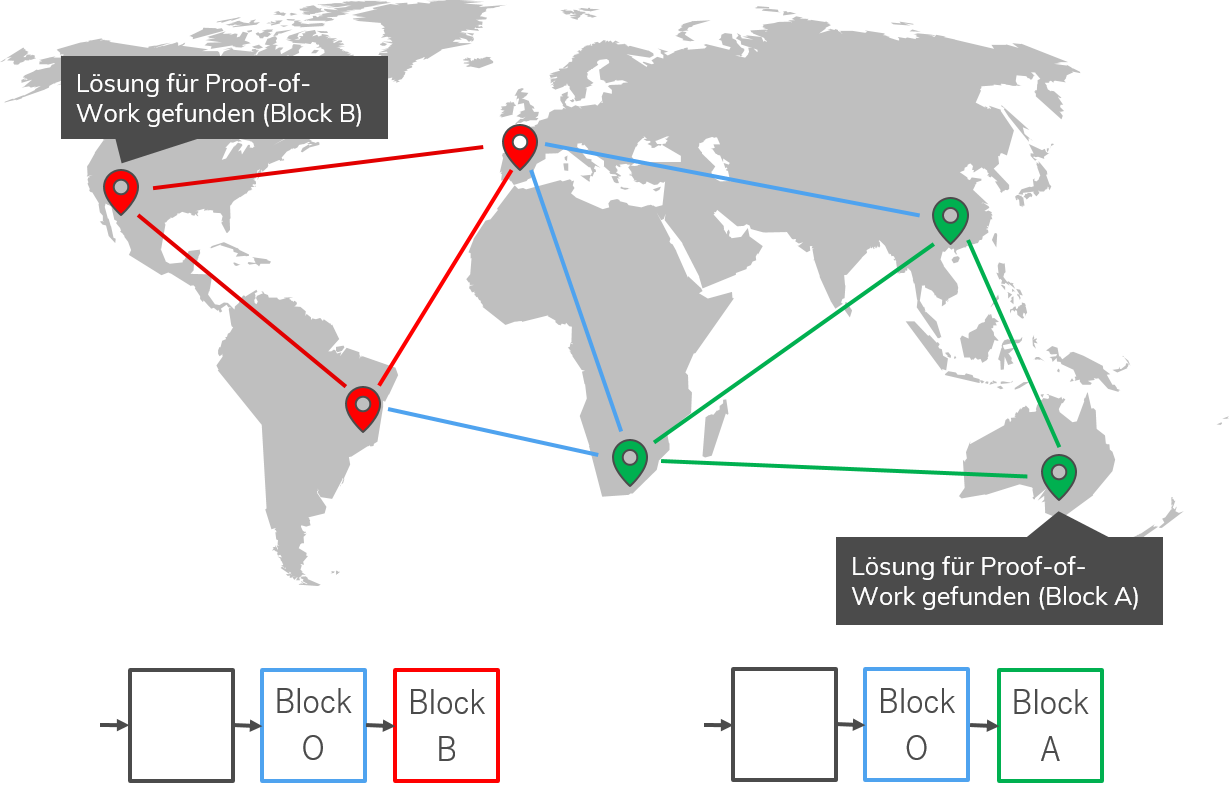
\includegraphics[width=0.95\textwidth,angle=0]{images/fork_2}
 	\caption{Fork-Visualisierung - zwei Nodes finden zur ungefähr gleichen Zeit einen Block und verbreiten ihn im Netzwerk, wodurch zwei Versionen der Blockchain bestehen \cite[S.~200 ff.]{AntonopoulosMasteringbitcoin2015}.}
	\label{fig:fork_2}
\end{figure}

\begin{figure}[!htbp]
  \centering
	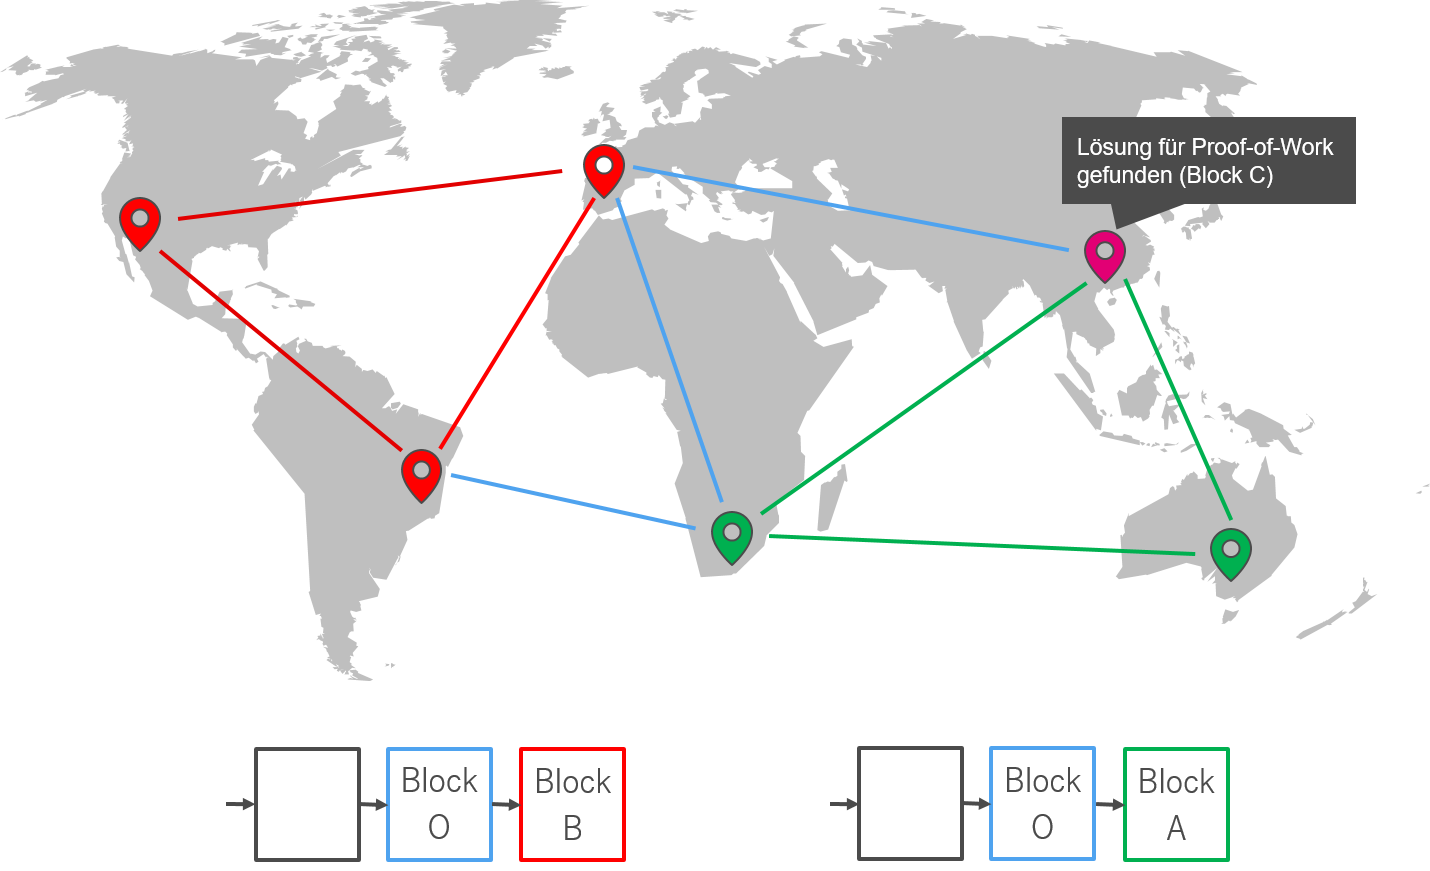
\includegraphics[width=0.95\textwidth,angle=0]{images/fork_3}
 	\caption{Fork-Visualisierung - Eine Node, welche Block A zuerst erhalten hat, hängt daran einen neuen Block C an \cite[S.~200 ff.]{AntonopoulosMasteringbitcoin2015}.}
	\label{fig:fork_3}
\end{figure}

\begin{figure}[!htbp]
  \centering
	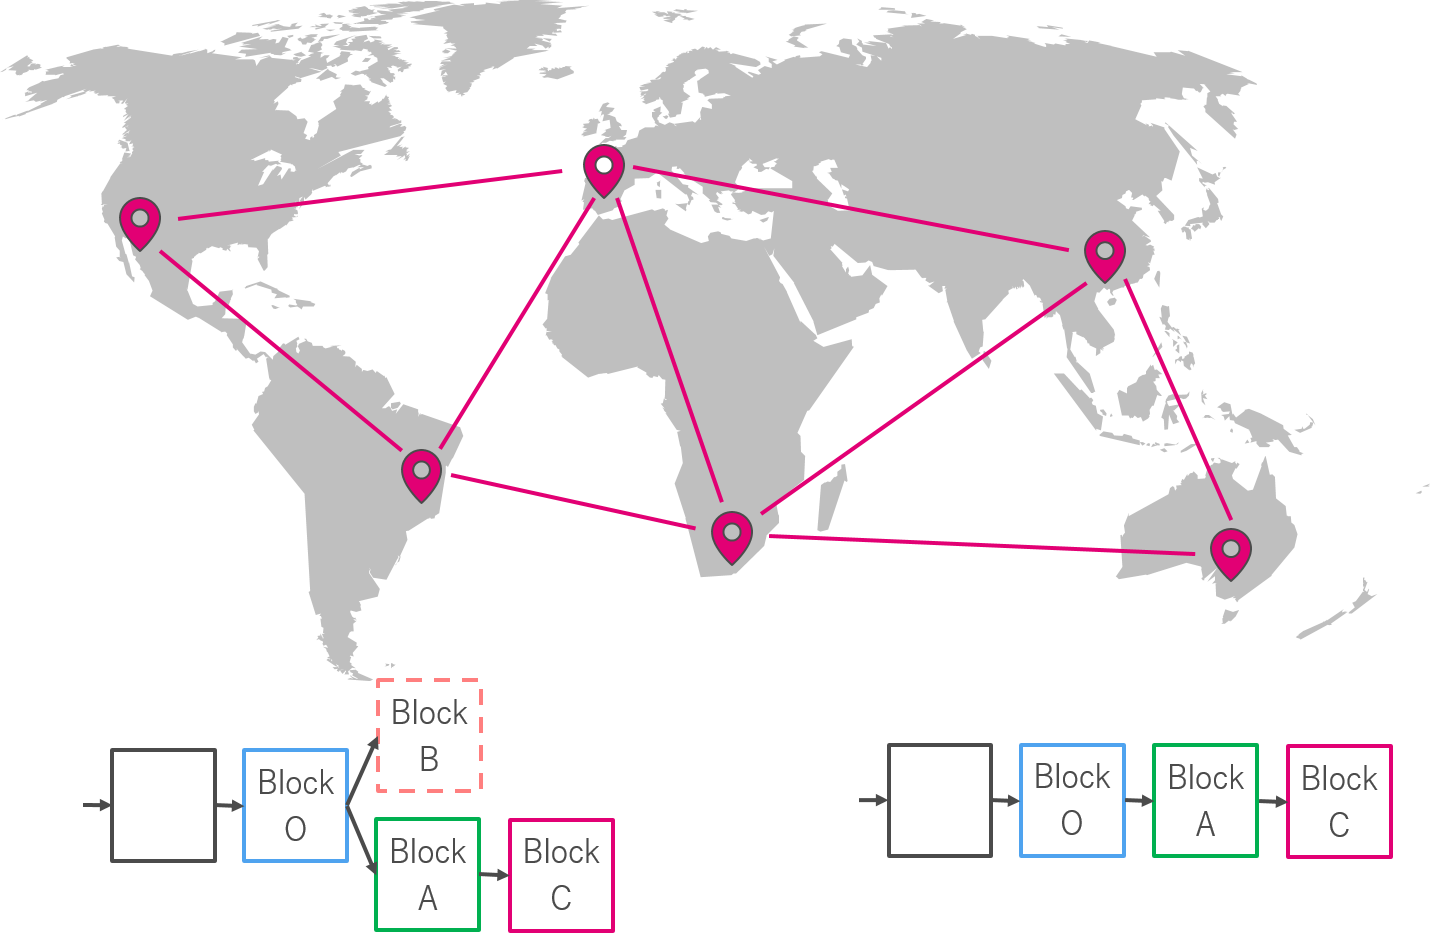
\includegraphics[width=0.95\textwidth,angle=0]{images/fork_4}
 	\caption{Fork-Visualisierung - Block C verbreitet sich im Netzwerk, rote Nodes sehen zwei Blockchains und akzeptieren die längere \cite[S.~200 ff.]{AntonopoulosMasteringbitcoin2015}.}
	\label{fig:fork_4}
\end{figure}

Neben dem \acs{PoW} gibt es noch weitere Konsensmechanismen, wie Proof-of-Stake, Proof-of-Authority oder Practical Byzantine Fault Tolerance \cite{SukhwaniPerformanceModelingPBFT2017a}, \cite{DeAngelisPBFTvsproofofauthority2017} . Diese werden im Kapitel \ref{sec:eval-konsens} genauer beschrieben und analysiert.

\subsubsection{Nichtangreifbarkeit und Unveränderlichkeit}
\label{subsec:immutability}
Viele Faktoren tragen zur Nichtangreifbarkeit und Unveränderlichkeit (im weiteren Verlauf nur noch als Sicherheit bezeichnet) der Blockchain bei. Da alle Nodes die ausgeführten Transaktionen auf Validität prüfen, können diese nicht ohne Berechtigung, im Namen einer anderen Identität oder mit unzureichenden Konditionen ausgeführt werden. Der wichtigste Faktor ist jedoch der genutzte Konsensmechanismus in Verbindung mit den verketteten Blöcken. Durch ihn wird sichergestellt, dass bestehende Daten nicht gelöscht oder manipuliert werden können.

Ein Beispiel dafür kann am \acs{PoW} gezeigt werden. Ein Angreifer probiert eine Transaktion aus einen bestehenden Block zu entfernen. Dazu würde er die Transaktion bei seiner lokalen Blockchain entfernen. Nun ist jedoch der Hash des Blockes sowie der Block selbst nicht valide und würde von keiner Node akzeptiert werden. Der Angreifer muss also erneut einen \acs{PoW} für den manipulierten Block erbringen. Dies wäre für eine Einzelperson jedoch zeitaufwändig. So benötigenm alle Nodes im Bitcoin-Netzwerk im Durchschnitt 10 Minuten, um einen \acs{PoW} zu erbringen \cite[S.~173]{AntonopoulosMasteringbitcoin2015}, bei einer Hash Rate\footnote{Hash Rate: Anzahl der in einer Zeiteinheit berechneten Hashwerte \cite{BitcoinTeamBitcoinGlossar}.} von ca. 13.000.000 TH/s (Terrahashes pro Sekunde) \cite{EtherscanEthereumNetworkHashRate}. Spezielle Hardware für das Mining erreicht hingegen nur eine Hashrate von bis zu 13,5 TH/s \cite{BitcoinminingLearnBitcoinmining}. Wenn der manipulierte Block nun noch Nachfolger hat, muss aufgrund des geänderten Hashes, auch für diese der \acs{PoW} erbracht werden. Hinzu kommt, dass die Blockchain des Angreifers erst dann von allen Nodes akzeptiert wird, wenn sie länger ist, als die aktuell akzeptierte. Er müsste also schneller als das gesamte Bitcoin-Netzwerk Blöcke erschaffen können. Dies ist nur möglich, wenn er 51 \% der Rechenleistung des Netzwerks besitzt. Deshalb wird dieser Angriff auch 51\%-Angriff genannt \cite[S.~83]{SwanBlockchainblueprintnew2015} \cite{EthereumTeamEthereumWhitePaper2017}. 

An dieser Stelle sollte erwähnt werden, dass, auch wenn ein 51\%-Angriff erfolgt, die Angriffsmöglichkeiten beschränkt sind. Der Angreifer kann keine invaliden Transaktionen sowie Blöcke erstellen. Ihm ist es möglich DoS-Angriffe auszuführen, indem er verhindert, dass bestimmte Transaktionen in Blöcken aufgenommen werden. Ebenso kann er die Historie der Daten verändern, indem er eine Transaktion aus einem Block entfernt. Es ist jedoch zu bedenken, dass die Transaktion dabei zurück in den Transaktionspool geht. Er muss also jeden weiteren Block erstellen, um zu verhindern, dass die Transaktion nicht erneut in einen Block aufgenommen wird oder dafür sorgen, dass sie ungültig wird. Im Falle von Kryptowährungen wird ein solcher Angriff Double-Spending-Angriff genannt: Ein Angreifer sendet beispielsweise Bitcoins an einen Händler. Dieser wartet auf die Bestätigung der Transaktion in einen Block sowie auf nachfolgende Blöcke. So stellt er sicher, dass die Transaktion nicht in einem eventuell verworfenen Fork-Branch steht. Erst dann versendet er die Ware. Anschließend ersetzt der Angreifer die Transaktion durch eine Zahlung an sich selbst und erstellt die längere Blockchain. Somit wird die Transaktion an den Händler ungültig, wodurch er letztendlich doch kein Geld erhalten hat \cite{EthereumTeamEthereumWhitePaper2017}. Auch zu bedenken ist, dass ein Nutzer mit 51 \% der Rechenleistung wenig Motivation hat Angriffe auszuführen, da er für jeden erstellten Block Kryptowährung als Belohnung erhält. Ebenfalls würde der Wert dieser sinken, wenn Angriffe auf die Blockchain entdeckt werden. Deshalb besteht für die sogenannten Miner eine Motivation, ehrlich zu arbeiten \cite[S.196 ff.]{AntonopoulosMasteringbitcoin2015}.

Der eben genannte Double-Spending-Angriff kann auf verschiedene Arten durchgeführt werden. So könnte ein Angreifer eine Ware mit Bitcoins bezahlen und diese sofort erhalten. Bevor seine Transaktion jedoch in einen Block besteht, transferiert er die gleichen Bitcoins an sein anderes Konto. Wenn diese beiden Transaktionen letztendlich in einen Block aufgenommen werden sollen, wird eine der Transaktionen ungültig sein, wodurch der Verkäufer eventuell keine Zahlung erhält \cite[S.~211 ff.]{AntonopoulosMasteringbitcoin2015}.

\subsection{Blockchaintypen}
Anhand der zugelassenen Teilnehmer an einer Blockchain ergeben sich 3 Typen. Bisher wurden nur Public Blockchain-Anwendungen, wie Bitcoin und Ethereum, erwähnt. In diesen gibt es keine Teilnehmerbeschränkungen, jeder kann am Netzwerk teilnehmen und die Blockchain öffentlich einsehen. Anders ist dies bei Permissioned (oder auch Consortium \cite{BenHamidaBlockchainEnterpriseOverview2017}) und Private Blockchains. Die beiden Begriffe werden in einigen wissenschaftlichen Arbeiten gleichgesetzt (siehe \cite{Gramolidangerprivateblockchains2016}, \cite{PongnumkulPerformanceAnalysisPrivate2017}, \cite{LiScalablePrivateIndustrial2017}). Hier folgt jedoch eine Unterscheidung. Dabei ist eine Private Blockchain eine Blockchain, welche nur von einem Nutzer verwendet wird. Da eine solche Anwendung keinen Sinn ergibt, da keine Vorteile der Blockchain genutzt werden können, wird darauf nicht genauer eingegangen. Interessanter sind Permissioned Blockchains, an welchen nur zugelassene Nutzer teilnehmen dürfen. Nur diese sind berechtigt, Transaktionen auszuführen und die Daten einzusehen \cite{LiScalablePrivateIndustrial2017}. Dies bietet sich vor allem bei B2B-Anwendungen an, welche von verschiedenen Unternehmen genutzt werden sollen. In solchen kann es beispielsweise aufgrund von sensiblen Daten nötig sein, dass nur bestimmte Parteien Zugriff auf die Blockchain haben. Tabelle \ref{tab:bc-comparison} vergleicht die Blockchaintypen untereinander sowie mit zentralen Datenbanken, da diese am häufigsten für persistente Datenspeicherung genutzt werden. Die dort erwähnten \acs{BFT}-Protokolle werden genauer im Kapitel \ref{sec:eval-konsens} erläutert.

\begin{table}[h]
    \centering
	\begin{tabular}{c c c c}
	\textbf{} & \textbf{Public BC} & \textbf{Permissioned BC}  & \textbf{Zentrale DB} \\ \hline
	Transaktionsdurchsatz & Gering & Hoch & Sehr hoch \\ \hline
    Nicht vertrauenswürdige Nodes & Viele & Wenige & Keine \\ \hline
    Konsensmechanismus & Hauptsächlich \acs{PoW} & \acs{BFT}-Protokolle & Keiner \\ \hline
    Zentral verwaltet & Nein & Teilweise & Ja \\
    \end{tabular}
    \caption{Vergleich der Blockchaintypen mit Datenbanksystemen \cite{WustyouneedBlockchain2017}\cite{ZhengBlockchainChallengesOpportunities2017}.}
	\label{tab:bc-comparison}
\end{table}

\subsection{Exemplarische Anwendungsfälle}
\label{subsec:use-cases}
Die Blockchain wird als revolutionäre Technologie angepriesen (siehe \cite{TapscottBlockchainRevolutionWieTechnologie2016}). Trotzdem ist es wichtig zu wissen, für welche Zwecke sie wirklich geeignet ist. Grundsätzlich ergibt eine Blockchain Sinn, wenn mehrere Parteien, welche sich nicht vertrauen, mit einem System interagieren wollen, welches von keiner dritten, zentralen Instanz verwaltet wird \cite{WustyouneedBlockchain2017}. Um eine bessere Vorstellung von solchen Anwendungen zu erhalten, werden im Folgenden verschiedene exemplarische Anwendungsfälle genannt und beschrieben.

Der erste Anwendungsfall, mit welchem die Blockchain-Technologie auch entstanden ist, sind Kryptowährungen. Mit Ihnen ist es möglich Geld zwischen beliebigen Parteien zu übertragen, ohne dass die Transaktionen von einer eventuell nicht vertrauenswürdigen Bank oder Ähnlichem kontrolliert und verwaltet werden \cite[S.~\Rn{10}]{SwanBlockchainblueprintnew2015}.

Weitere Anwendungsfälle ergeben sich mit der Möglichkeit, Programmlogik auf der Blockchain abzubilden. So können beispielsweise dezentrale Online-Wahlen realisiert werden. Die Stimmen würden in der Blockchain gesammelt werden und können so letztendlich nicht mehr manipuliert werden, beispielsweise von einer korrupten Regierung \cite{CastorEthereumVotingScheme2017}. 

Ein weiterer Anwendungsfall, insbesondere für den B2B-Bereich, wäre Supply Chain Management. Über eine digitale Lieferkette sollen Material- und Informationsflüsse zu Produkten und Dienstleistungen aufgebaut und verwaltet werden \cite{KriegerSupplyChainManagement}. Dies erlaubt Unternehmen das Automatisieren von Prozessen und das verbesserte Reagieren auf Ereignisse (z. B. Lieferverspätungen). Weiterhin ist es dem Unternehmen möglich, dem Kunden exakt aufzuzeigen, wo das Produkt und seine Unterprodukte produziert wurden. In klassischen B2B-Anwendungen müsste jedes Unternehmen, welches ein Teil der Supply Chain ist, die relevanten Daten beispielsweise durch APIs\footnote{API: Schnittstelle für Anwendungsprogrammierung\cite{DigHowAPIsevolve2006}.} bereitstellen. Dies ist mit großen Aufwand verbunden, da diese erstmal entwickelt werden müssen. Weiterhin müssten Plattformen die Daten von unterschiedlichen Schnittstellen abfragen, um diese zusammenzuführen. Aufgrund dieses Aufwandes werden oft Dritte eingestellt, welche sich um den Aufbau und um die Datenintegration der Supply Chain kümmern. Den Aufwand sowie die eventuell nicht vertrauenswürdige dritte Partei könnte durch die Nutzung der Blockchain eliminiert werden. In dieser könnte jedes Unternehmen die relevanten Daten an einer Stelle speichern. Die Supply Chain wäre direkt in der Blockchain vorhanden und kein Unternehmen muss Datenmanipulation oder Ähnliches befürchten \cite{KorpelaDigitalSupplyChain2017}.

Auch dezentrale Märkte sind für B2B-Anwendungen interessant. Der zentrale Marktplattformbetreiber (z. B. Ebay oder Amazon), welcher persönliche Informationen speichert und Gebühren für den Verkauf von Artikeln verlangt, wäre hinfällig. Nutzer könnten Waren untereinander verkaufen, während die Blockchain als Notar für den Warenaustausch dient \cite{BenHamidaBlockchainEnterpriseOverview2017}.

Ein weiteres Beispiel wären Blockchain Sharing-Systeme. So könnte ein dezentrales Fahr-radleihsystem aufgebaut werden. Nutzer würden mit ihrem Smartphone, über ihre in der Blockchain hinterlegte Identität (im Falle von beispielsweise Ethereum die Wallet-Adresse\footnote{Wallet: Speichert beispielsweise bei Ethereum und Bitcoin den Private Key des Nutzers und wird als Adresse für Zahlungen genutzt \cite[S.~61 ff.]{AntonopoulosMasteringbitcoin2015}.}), das Fahrrad entsperren. Dieses erkennt automatisch die gefahrene Distanz sowie die Nutzungsdauer. Über einen Smart Contract würde anschließend die automatische Zahlung erfolgen. Neben der Automatisierung besteht der Vorteil, dass mehrere Unternehmen oder auch Privatpersonen Leihfahrräder anbieten können, ohne dass sie einer zentralen Instanz mit der Verwaltung vertrauen müssen \cite{FutureFluxFestivalBlockchainBikes}, \cite{FischerIoTBlockchain}.

\section{Anforderungen an B2B-Anwendungen}
\label{sec:general-requirements}
Für den zu entwickelnden Prototypen ergeben sich verschiedene Anforderungen, welche zum Teil allgemein für B2B-(Blockchain)-Anwendungen gelten. Es ist wichtig diese zu kennen, um die Blockchain-Technologie in Bezug auf diese zu evaluieren.

\paragraph{Identitätsverwaltung}
Eine B2B-Anwendung besteht zwischen verschiedenen Unternehmen. Die Identitäten dieser müssen bekannt sein, um die Teilnahmeerlaubnis zu erteilen und Berechtigungen zu verwalten. Sie sind ebenfalls von Bedeutung, um ausgeführte Transaktionen den Teilnehmern zuordnen zu können. Die für den Prototypen genutzte Blockchain-Implementierung muss also das Registrieren und Identifizieren von Teilnehmern unterstützen.

\paragraph{Berechtigungsverwaltung}
Die verschiedenen Teilnehmer haben unterschiedliche Rechte was das Lesen, Erstellen und Verändern von Daten betrifft. So ist es beispielsweise wichtig, dass ein Teilnehmer nur seine eigenen, in der Blockchain registrierten, Assets\footnote{Assets: Besitz/Eigentum} verändern kann.

\paragraph{Private Transaktionen}
Bei Blockchains wie Bitcoin und Ethereum sind alle Daten in der Blockchain für alle Teilnehmer einsehbar. Aufgrund von sensiblen Daten kann es allerdings vorkommen, dass nicht alle Transaktionen für alle Teilnehmer sichtbar sein sollen. So sollen beispielsweise Preisabsprachen nur von den relevanten Unternehmen eingesehen werden können.

\paragraph{Skalierbarkeit und Performance}
In Bitcoin ist lediglich ein Transaktionsdurchsatz von 7 \acl{TPS} (\acs{TPS}) möglich \cite{ZhengBlockchainChallengesOpportunities2017}. Hinzu kommt, dass es ca. zwischen 30 Minuten und 16 Stunden dauern kann, bis eine Transaktion bestätigt ist \cite{BuchkoHowLongBitcoin2017}. Darauf wird auch genauer im Kapitel \ref{sec:scalability-eval} eingegangen. In B2B-Anwendungen kann die Performance und Skalierbarkeit von großer Bedeutung sein. Je nach Art der Anwendung und Anzahl der Teilnehmer muss ein höherer Transaktionsdurchsatz als bei Bitcoin erzielt werden. Die Skalierbarkeit ist vor allem beim Einsatz von IoT-Geräten von Bedeutung, welche untereinander kommunizieren und Transaktionen ausführen. Gartner behauptet, dass es bis 2020 ca. 7,5 Billionen vernetzte Geräte im Business-Sektor geben wird \cite{RobGartnerSaysBillion2017}. Damit wäre ein Transaktionsdurchsatz von 7 TPS nicht praktikabel.

\paragraph{Sicherheit}
Die Sicherheit wird durch den genutzten Konsensmechanismus realisiert. Der am häufigsten genutzte \acs{PoW} ist in einem Netzwerk mit wenig Teilnehmern allerdings unsicher, da es einfach ist 51 \% der Rechenleistung zu erreichen. Weiterhin führt er zu einen hohen Stromverbrauch (im Bitcoin-Netzwerk der Verbrauch von ca. 3.500.000 US-Haushalten \cite{DigiconomistBitcoinEnergyConsumption}), welcher nicht erwünscht ist. Ebenfalls beeinflusst der \acs{PoW} die Performance (siehe Kapitel \ref{cha:b2b-eval}).



	
\chapter{Dezentraler Wartungsmarkt - Konzept}
\label{cha:fazit}

\section{Allgemein}
Ziel dieser Arbeit ist die Entwicklung einer prototypischen B2B-Applikation in Form eines automatisierten sowie dezentralisierten Wartungsmarktes. Teilnehmer an diesem sind multiple Unternehmen und Wartungsanbieter. Erstere besitzen IoT-Geräte, welche erkennen können, dass sie eine Wartung benötigen. Die Wartungsanbieter erhalten die Informationen zur Wartung, und können sich für diese anmelden. Anschließend würden sie diese durchführen und dabei die Wartungsschritte loggen.  

In klassischen B2B-Anwendungen wäre die Realisierung dieses Systems auf 2 Arten erfolgt. Bei ersterer gäbe es eine dritte Partei, welche den Markt verwaltet, und bei welcher sich alle Unternehmen und Wartungsanbieter anmelden müssen (z.B. Ebay). Die andere Möglichkeit wäre, dass eines der teilnehmenden Unternehmen den Markt verwaltet. Bei beiden Optionen müssten die Teilnehmer am Markt ihre Daten einer eventuell nicht vertrauenswürdigen zentralen Instanz zur Verfügung stellen. Weiterhin würde bei jeden Unternehmen die Notwendigkeit bestehen, API's für den Datenzugriff zu erstellen.

Um dies zu verhindern, wird der Wartungsmarkt auf Basis der Blockchain-Technologie implementiert. Somit können beliebig viele Unternehmen und Wartungsanbieter an dem System teilnehmen, ohne dass eine Datenmanipulation durch die Teilnehmer oder eine zentrale Instanz befürchtet werden muss.

%TODO: Formatierung des Kapitels bearbeiten ?

%TODO: S.3 WustYouNeed: Flowchart for choosing a blockchain type --> Connection to our system 
\section{Anforderungen}
Es ergeben sich verschiedene Anforderungen an das zu entwickelnde System. Die Spezifizierung dieser ist wichtig, denn auf Basis von diesen wird eine Blockchain-Implementation ausgewählt und auf verschiedene Probleme analysiert. Dieser werden hier zunächst einmal aufgelistet um einen Überblick zu erhalten.

%TODO: Alles durch Paragraphs ersetzen
Es ergeben sich verschiedene funktionale Anforderungen:
\begin{itemize}
    \item Registrieren und Identifizieren von Unternehmen, Wartungsanbietern und Geräten in der Blockchain
    \item Wartungsgeräte kündigen Wartungen in Form eines Smart Contracts in der Blockchain an
    \item Wartungsanbieter können den Smart Contract unter bestimmten Konditionen annehmen
    \item Wartungsanbieter loggen Wartungsschritte in der Blockchain
    \item Gerät überprüft ob die Wartung erfolgt ist, und schließt den Contract
    \item Nur bestimmte Teilnehmer können bestimmte Transaktionen ausführen
    \item Private Transaktionen sollen zwischen Teilnehmern möglich sein
\end{itemize}

%TODO: Hier nochmal erwähnen, dass die Daten dezentral, unmanipulierbar, ohne zentral verwaltene Instanz gespeichert werden sollen ?
Folgende nicht-funktionale Anforderungen existieren:

\begin{itemize}
    \item Hoher Transaktionsdurchsatz und geringe Transaktionszeiten
    \item Nichtangreifbarkeit der Daten
\end{itemize}

Einige Anforderungen sollten genauer erklärt werden:

\begin{quote}
    ``Registrieren und Identifizieren von Unternehmen, Wartungsanbietern und Geräten in der Blockchain''
\end{quote}

Die zu entstehende B2B-Anwendung soll zwischen verschiedenen Unternehmen bestehen. Diese müssen Berechtigungen erhalten um am Netzwerk teilzunehmen, und ausgeführte Transaktionen sollen ihnen zugeordnet werden können.

\begin{quote}
    ``Wartungsgeräte kündigen Wartungen in Form eines Smart Contracts in der Blockchain an''
\end{quote}

Es kann verschiedene Gründe für die Wartung geben. So kann z.B. ein Wartungsdatum erreicht werden, oder Sensorwerte weisen auf einen Fehler hin.

\begin{quote}
    ``Wartungsanbieter können den Smart Contract unter bestimmten Konditionen annehmen''
\end{quote}

Eine dieser Konditionen könnte sein, dass der Wartungsanbieter bereits Erfahrungen mit der Wartung von bestimmten Geräten hat. Diese Information könnte ebenfalls aus der Blockchain abgefragt werden. Weiterhin darf der Vertrag z.B. noch nicht von einen anderen Anbieter akzeptiert worden sein. 

\begin{quote}
    ``Gerät überprüft ob Wartung erfolgt ist, und schließt den Contract''
\end{quote}

Die Überprüfung kann anhand der geloggten Schritte sowie Sensorwerten erfolgen, welche vor und nach der Wartung existiert haben.

\begin{quote}
    ``Nur bestimmte Teilnehmer können bestimmte Transaktionen ausführen''
\end{quote}

Die verschiedenen Teilnehmer haben unterschiedliche Rechte. So soll es z.B. einen Unternehmen nicht möglich sein, Wartungsverträge zu bearbeiten oder zu akzeptieren.

\begin{quote}
    ``Private Transaktionen sollen zwischen Teilnehmern möglich sein''
\end{quote}

Bei Blockchains wie Bitcoin und Ethereum sind alle Daten in der Blockchain für alle Teilnehmer einsichtbar. Aufgrund von sensiblen Daten kann es allerdings vorkommen, das nicht alle Transaktionen für alle Teilnehmer sichtbar sein sollen. Im Falle des Wartungsmarktes sollen z.B. Preisabsprachen zwischen Unternehmen und Wartungsdienstleistern privat erfolgen.

%TODO: Daten aus Paper ? Skalierung IoT-Geräte ?
\begin{quote}
    ``Hoher Transaktionsdurchsatz und geringe Transaktionszeiten''
\end{quote}

In Bitcoin ist lediglich ein Transaktionsdurchsatz von 7 Transaktionen pro Sekunde möglich \cite{ZhengBlockchainChallengesOpportunities2017}. Hinzu kommt, dass es ca. zwischen 30 Minuten und 16 Stunden dauern kann, bis eine Transaktion bestätigt ist \cite{BuchkoHowLongBitcoin2017}. Darauf wird auch genauer im Kapitel \ref{sec:scalability-eval} eingegangen. In dem zu entwickelnden System ist die Skalierbarkeit wichtig. Je nach der Anzahl der am Netzwerk teilnehmenden Unternehmen und Wartungsanbieter wird eine höherer Transaktionsdurchsatz benötigt. Insbesondere wenn tausende von Geräten Transaktionen in der Blockchain ausführen.

\begin{quote}
    ``Nichtangreifbarkeit der Daten''
\end{quote}

Die Nichtangreifbarkeit wird durch die genutzte Konsensmechanik realisiert. Der am häufigsten genutzte Proof-of-Work ist in einem Netzwerk mit wenig Teilnehmern allerdings unsicher, da es einfach ist 51\% der Rechenleistung zu erreichen. Weiterhin führt er zu einen hohen Stromverbrauch (Im Bitcoin-Netzwerk der Verbrauch von ca. 3.500.000 US-Haushalten \cite{BitcoinEnergyConsumption}), welcher nicht erwünscht ist.

An dieser Stelle muss darauf hingewiesen werden, dass das System um viele nützliche Features erweiterbar ist. So könnte zum Beispiel eine Bewertung der Wartungsanbieter anhand bestimmter Faktoren erfolgen. Da es sich jedoch nur um eine prototypische Implementation handelt, werden nur die Features implementiert, welche für einen Proof-of-Concept eines solchen Systems benötigt werden.



%TODO: Rename
\chapter{Aktueller Stand der Technik}
\label{cha:stand-technik}

Die Blockchain wird seit 2008 erfolgreich für Kryptowährungen eingesetzt. Mit Ethereum wird das Konzept von Smart Contracts implementiert, womit es möglich ist eigene Programmlogik in der Blockchain abzubilden und so dezentrale Anwendungen zu entwickeln. Weitere weniger bekannte Blockchain-Implementationen für Public Blockchains sind Monero, Dashcoin und Litecoin \cite{BlockchainHubBlockchainsDistributedLedger}. 

Die Technologie bringt durch ihre Architektur jedoch auch Limitationen mit sich, weshalb sie nicht für alle Anwendungszwecke geeignet ist (Siehe \ref{cha:b2b-eval}. Die Probleme werden in vielen wissenschaftlichen Arbeiten analysiert und Lösungen für diese vorgeschlagen. Trotzdem bestehen gewisse Limitationen weiterhin \cite{ZhengBlockchainChallengesOpportunities2017}\cite{SwanBlockchainblueprintnew2015}\cite{SchererPerformanceScalabilityBlockchain2017}.

Permissioned Blockchains, wie Hyperledger Fabric, Quorum, Sawtooth Lake oder Quorum bieten Vorteile gegenüber dem Public Blockchains, sie bringen allerdings auch neue Herausforderungen mit sich. So muss z.B. eine Alternative zum Proof-of-Work gefunden werden, um je nach Use-Case, Performance, Skalierbarkeit und Nichtangreiffbarkeit sicher zu stellen \cite{LiScalablePrivateIndustrial2017}.

Dezentrale Märkte sind eine der am meisten mit Blockchain in Verbindung erwähnten Use-Cases, wie man an Quellen wie \cite{BenHamidaBlockchainEnterpriseOverview2017} und \cite{RavalDecentralizedApplicationsHarnessing2016} sehen kann.
Neben Konzepten für diese (Siehe \cite{KaiserDecentralizedPrivateMarketplace}), gibt es auch Live-Systeme, wie Syscoin \cite{SidhuSyscoinPeertoPeerElectronic2017}.

Dezentrale Wartungsmärkte hingegen werden nur in Verbindung mit der Supply Chain erwähnt, wie zum Beispiel in \cite{SoldatosWhatDoesBlockchain} oder \cite{GotzeLufthansaIndustrySolutions}. Implementationen oder Konzeptentwürfe konnten nicht gefunden werden.





\chapter{Evaluierung Permissioned Blockchains für B2B}
\label{cha:b2b-eval}

Die Blockchain-Technologie bringt diverse Probleme mit sich, welche je nach Anwendungszweck und Blockchaintyp verschieden große Auswirkungen haben. Für den B2B-Bereich gilt es vor allem die Skalierbarkeit sowie die Konsensmechanismen zu analysieren.


\section{Skalierbarkeit}
\label{sec:scalability-eval}
Das CAP-Theorem besagt, dass es in einem verteilten System nur möglich ist, 2 von den 3 folgenden Eigenschaften zu erfüllen: Konsistenz, Verfügbarkeit und Ausfalltoleranz. Bei der Blockchain wären dies: Dezentralisierung, Skalierbarkeit und Nichtangreifbarkeit \cite{SchererPerformanceScalabilityBlockchain2017}. Im Bezug auf die Skalierbarkeit wird vor allem auf den Transaktionsdurchsatz sowie die Bestätigungszeiten von Transaktionen eingegangen. Dazu erfolgt zunächst eine Analyse an aktuellen Public Blockchains, und letztendlich an Permissioned Blockchains. Die Ergebnisse werden ebenfalls auf das CAP-Theorem angewandt.  

\subsection{Public Blockchains}

\begin{figure}[htb]
  \centering
    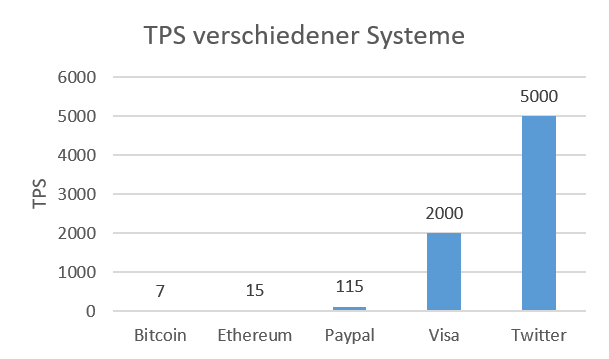
\includegraphics[width=0.95\textwidth,angle=0]{images/tps-comparison}
     \caption{Möglicher Transaktionsdurchsatz bei Bitcoin, Ethereum, Paypal und Visa \cite{ScalabilityBitcoinWiki}.}
    \label{fig:tps-comparison}
\end{figure}

%TODO: Bitcoin-Kapitel nochmal unterteilem in paragraphs ?
\subsubsection{Bitcoin}
%TODO: Transaktionsgebühren erwähnen ?
Das Bitcoin-Netzwerk erreicht aktuell einen maximalen Transaktionsdurchsatz von 7 Transaktionen (Unterschiedlich je nach Größe der Transaktionen) pro Sekunde (TPS), bei einer Blockgröße von 1MB.  Hingegen erreicht Paypal 115 TPS, und Visa 2000 TPS (Siehe auch Abb. \ref{fig:tps-comparison}) \cite{ScalabilityBitcoinWiki}. Hinzu kommt, dass ungefähr 170000 unbestätigte Transaktionen\footnote{Unbestätigte Transaktion: Eine Transaktion, welche noch nicht in einen Block vorkommt \cite{AntonopoulosMasteringbitcoin2015}} bestehen \cite{BlockchainFirmaBlockchainChartsUnbestatigte}. Berechnungen von Scherer zeigen, dass bei 11,8 Millionen Nutzern im Bitcoin-Netzwerk, sowie einem Transaktionsdurchsatz von 4 TPS, jeder Nutzer nur nur ca. 10 Transaktionen im Jahr senden kann \cite{SchererPerformanceScalabilityBlockchain2017}.

%TODO: SegWit ?
Der Transaktionsdurchsatz ist durch verschiedene Faktoren limitiert. Hauptsächlich durch die limitierte Blockgröße von 1MB, und dem Proof-of-Work: Nur eine bestimmte Anzahl an Transaktionen passt in einen Block, und nur alle 10 Minuten wird einer erstellt. Es gäbe also die Möglichkeit, die Blockgröße zu vergrößern, oder die Zeit für den Proof-of-Work zu verringern, indem die Schwierigkeit angepasst wird. Es gibt jedoch diverse Nachteile, welche dadurch entstehen würden. Bei einer größeren Blockgröße würde es länger dauern, bis ein Block beim Propagieren durch das Netzwerk alle Nodes erreicht. Dies würde zu öfter vorkommenden und längeren Forks führen und somit die Sicherheit des Netzwerks beeinträchtigen. Den gleichen Effekt hätte eine kürzere Proof-of-Work Zeit, da die Wahrscheinlichkeit höher ist, dass zwei Nodes zur ungefähr gleichen Zeit einen Block erstellen \cite{SchererPerformanceScalabilityBlockchain2017} \cite{EthereumWhitepaper2017} \cite{SompolinskyAcceleratingBitcoinTransaction2013}. 

%TODO: Erhöhte Chance auf Angriff/Double Spend erwähnen ?
Entsteht ein Fork, probieren Nodes die längere und somit gültige Blockchain zu erschaffen. Gelingt dies, wird die kürzere Blockchain mit den nun sogenannten Stale Blocks verworfen. Die gesamte Rechenleistung, welche in die Stale Blocks und seine Nachfolger geflossen ist, trägt nicht zur Sicherheit des Netzwerks bei. Dies lässt sich auch anhand der Abbildung \ref{fig:forking-risks} erläutern. Innerhalb der Blockchain bestehen durch mehrere Forks 5 Branches. Das bedeutet, dass die Rechenleistung des Netzwerks auf diese aufgespalten ist. Es wird davon ausgegangen, dass 20\% der Rechenleistung in den obersten Branch geflossen ist, welcher der längste ist. Die restlichen 4 Branches erhalten je 10\% der Rechenleistung. Wenn es nun einen Angreifer mit 40\% der Rechenleistung probiert eine eigene Blockchain zu erstellen, gelingt ihm dies, da er schneller die längere Blockchain erstellen kann \cite{SompolinskyAcceleratingBitcoinTransaction2013}. Zusammenfassend lässt sich sagen, dass ein Angreifer nicht 51\% der Rechenleistung für einen Fork benötigt, wenn das Netzwerk diese bei Forks verschwendet \cite{Buterin12secondBlockTime2014}. 

Ein weiteres Problem der Forks ist, dass Miner keine Belohnung für die Arbeit an verworfenen Blöcken erhalten. Dadurch kann es zur Zentralisierung durch wachsende Mining Pools kommen. Dies wird an folgenden Beispiel ersichtlich: Ein Mining Pool A besitzt 30\% der Rechenleistung, ein Mining Pool B 10\%. In dem genannten Beispiel würde Mining Pool A in 70\% aller Fälle einen Stale Block erzeugen, und B in 90\% aller Fälle. Kein Miner würde dem Mining Pool B beitreten, da die Wahrscheinlichkeit geringer ist, dass B gültige Blöcke erschafft. A hingegen würde immer mehr Miner, und somit mehr Rechenleistung erhalten \cite{EthereumWhitepaper2017}.

%TODO: Quelle
%TODO: Benachteiligung von Minern erwähen ?
%Ein weiterer wichtiger Punkt in Bezug auf die Propagationszeiten ist die Benachteiligung von Minern.  Nodes, welche neue Blöcke erst später erhalten, können erst später mit dem Mining beginnen. Dazu ein Beispiel: Ein Miner A besitzt 45\% der Rechenleistung und es dauert 4 Sekunden bis ein Block bei allen anderen Nodes angekommen ist. Alle 5 Sekunden entsteht ein neuer Block. A wird in 45\% aller Fälle einen Block an die Blockchain anhängen. Er kann direkt mit den minen des neuen Blocks anfangen, während alle anderen Nodes erst nach 4 Sekunden erfahren, dass bereits ein neuer Block gefunden wurde. Alle anderen Nodes hätten somit nur noch 1 Sekunde um einen neuen Block an diesen anzuhängen. Somit würde hauptsächlich A Blöcke erstellen, und damit die Kontrolle über das Netzwerk haben.

An dieser Stelle sollte auch darauf hingewiesen werden, dass schnellere Blockerstellungszeiten nicht zwingend zu schnelleren Transaktionsbetätigungen führen. Transaktionen werden zwar schneller in Blöcken aufgenommen, aber es muss auf mehr Nachfolger gewartet werden, um sicher zu gehen, dass die Transaktion nicht in einem Fork vorkommt \cite{SchererPerformanceScalabilityBlockchain2017}.

\subsection{Ethereum}

\paragraph{Bessere Skalierbarkeit durch GHOST}
Das Ethereum Netzwerk nutzt das sogenannte GHOST-Protokoll, und erreicht damit eine Transaktionsdurchsatz von 15 TPS, bei einer durchschnittlichen Zeit von 15 Sekunden um den Proof-of-Work zu erbringen. Dieses löst Probleme des Forkings und der Benachteiligung von Minern. Ersteres wird dadurch gelöst, dass Stale Blocks in die Berechnung der gültigen Blockchain einfließen. Anders als bei Bitcoin, wo lediglich die Parents und deren Nachfolger eine Rolle spielen. Die Stale Blocks werden in Ethereum ``Uncles'' genannt. Kurz gesagt, ist ein Uncle ein alternativer gefundener Block welcher auf der gleichen Höhe wie der Parent bestehen würde \cite{EthereumWhitepaper2017}.

Die Bestimmung der gültigen Blockchain wird an der Abbildung \ref{fig:forking-risks} ersichtlich. In Ethereum ist die Blockchain die gültige, für welche die meiste Arbeit aufgebracht wurde, unter Einbezug der Uncles. Das führt dazu, dass der Branch mit den meisten Uncles bestehen bleibt. Das bedeutet letztendlich, dass die gesamte Rechenleistung das Netzwerk absichert, auch wenn diese sich auf die Branches aufteilt. Ein Angreifer braucht somit weiterhin 51\% der Rechenleistung um einen Angriff auszuführen \cite{SompolinskyAcceleratingBitcoinTransaction2013}.

Damit ist allerdings noch nicht das Problem der Zentralisierung durch Mining Pools gelöst. Es besteht weiterhin keine Motivation für Miner, Uncles zu minen. Deswegen ist das GHOST-Protokoll in Ethereum so erweitert, dass Miner Ether\footnote{Kryptowährung von Ethereum \cite{EthereumWhitepaper2017}.} als Belohnung für das Erstellen von Uncles erhalten (Allerdings weniger als bei vollwertigen Blöcken). Somit besteht ebenfalls die Motivation, kleineren Mining Pools beizutreten \cite{EthereumWhitepaper2017}. An dieser Stelle sollte auch erwähnt werden, dass Miner entscheiden können, an welchen Branch sie arbeiten \cite{ZhengBlockchainChallengesOpportunities2017}.

Während Ethereum die Probleme löst, welche durch Forks entstehen, ist der Transaktionsdurchsatz trotzdem limitiert. Die Blockgröße muss klein genug bleiben, damit das Propagieren im Netzwerk effizient bleibt \cite{SchererPerformanceScalabilityBlockchain2017}. Ansonsten würden Miner unter Umständen so benachteiligt werden, dass Sie nur noch Uncles minen können. Allerdings sind diese nur gültig, wenn sie maximal eine bestimmte Anzahl an Generationen vom aktuellen Block in der gültigen Chain entfernt sind. Ansonsten hätten die Miner eventuell auch keine Intention ehrlich zu bleiben, da sie ohne Nachteile an der Chain eines Angreiffers arbeiten könnten \cite{EthereumWhitepaper2017}.

%Das Problem der Benachteiligung der Miner wird dadurch gelöst, dass es ihnen möglich ist zu entscheiden, ob sie einen neu gefunden Block ignorieren. Mit Bezug zum oberen Beispiel: Miner A, mit 45\% der Rechenleistung, findet einen Block und  alle anderen Nodes erhalten diesen nach 4 Sekunden. Die Wahrscheinlichkeit sehr gering ist, dass sie innerhalb von einer Sekunde einen Block finden welchen sie an den neuen anhängen können. Deshalb entscheiden sich die Nodes dazu den Block zu ignorieren, und arbeiten mit 55\% der Rechenleistung weiter am alten Block. Dies führt dazu, dass sie 

\paragraph{Schlechtere Skalierbarkeit durch Smart Contracts}
Ethereum löst die Probleme von häufig auftretenden Forks und erlaubt so einen höheren Transaktionsdurchsatz sowie schnellere Transaktionsbestätigungszeiten. Weitere Probleme entstehen jedoch, wenn eine Blockchain nicht nur Geldtransfertransaktionen verarbeitet. Ethereum erlaubt das speichern und ausführen von eigenem Code durch Smart Contracts. Dadurch steigt die Komplexität der auszuführenden Transaktionen. Die Skalierbarkeit und Performance des Netzwerks verschlechtern sich, da die Datenmengen und damit Blockgrößen ansteigen sowie jede Node den Code lokal ausführen muss um Konsens herzustellen \cite{SchererPerformanceScalabilityBlockchain2017}.

%TODO: S.23 Scherer: Ethereum Blocks have to be smaller to guarantee a fast enough propagation
%TODO: S.3 SchererPerformance: Every node validating every transaction causes bad performance 
%TODO: S.23 Scherer: Ethereum is worse off with scaling because of the complexity (Not only money transactions)
%TODO: Ethereum All Code executed on every node
%TODO: S.2 Gramoli R3 constorium with 45 banks (?)
%TODO: S.2-4 Vukolic More Limitations of Permissioned Blockchains (Code execution, Non Determininstic Execution, Execution on all nodes)   

\begin{figure}[htb]
  \centering
    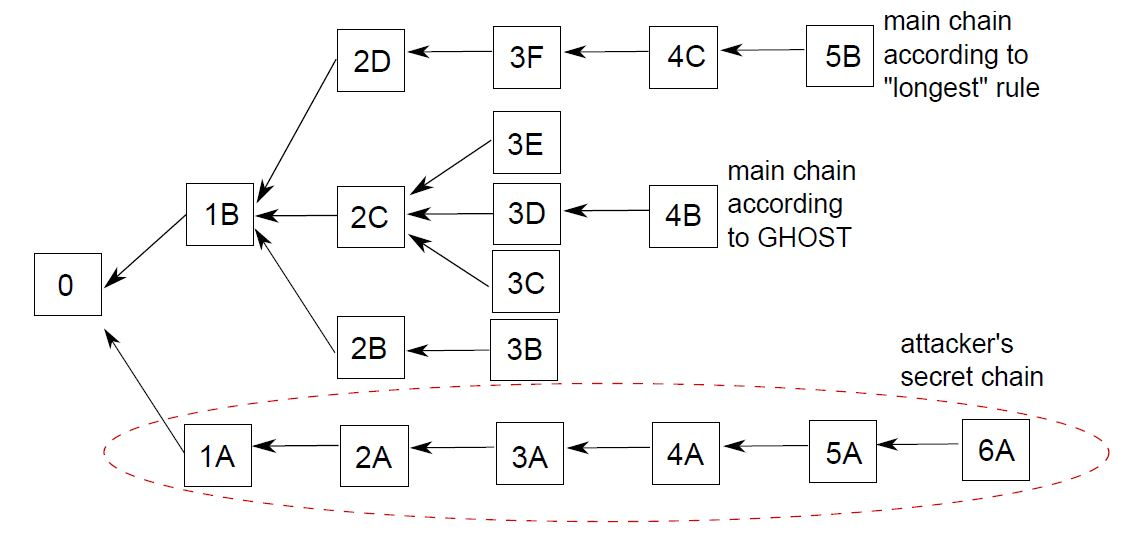
\includegraphics[width=0.8\textwidth,angle=0]{images/forking-risks}
     \caption{Auswahl der gültigen Blockchain. In Bitcoin die längere Blockchain. In Ethereum die Blockchain }
    \label{fig:forking-risks}
\end{figure} 

Letztendlich lässt sich sagen, dass Public Blockchains nicht skalieren \cite{SchererPerformanceScalabilityBlockchain2017}. Betrachtet man das CAP-Theorem wird ersichtlich, dass nur die Eigenschaften Dezentralisierbarkeit und Sicherheit gegeben sind. Weitere (teilweise gelöste ?) Schwierigkeiten gibt sobald nicht nur Geldtransferaktionen bestehen. Es ist jedoch zu bedenken, dass die meisten Probleme für die Skalierbarkeit aufgrund der genutzten Konsensmechanik bestehen. Auch wenn es teilweise Lösungsvorschläge für diese gibt, genügen sie bisher nicht um Skalierbarkeit herzustellen. Deshalb gilt es, die Probleme ebenfalls in Permissioned Blockchains zu analysieren. 

%TODO: Lightning Network
%TODO: S.23 Scherer: "The bottom line is that public networks are not efficient"
%TODO: MinPermissioned: Introduces a concept for better throughput, but it is not tested (??)
%TODO: S.1-6 LiScalable: Introducing a concept with sattelite chains

%Noch nicht angesprochen wurden Lösungen auf der Netzwerkebene, um die Blockverteilung zu beschleunigen (?). So könnte man die Netzwerktopologie verbessern \cite{}, oder das Lightning Network einsetzen. ... . Mit diesen wird sich hier im Detail jedoch nicht beschäftigt, denn in Permissioned Blockchains kann der Proof-of-Work nur unter bestimmten Voraussetzungen effizient und sicher eingesetzt werden, und ist damit eher unbrauchbar.

\subsection{Permissioned Blockchains}
Bezieht man sich auf das CAP-Theorem, müsste sich durch die stärkere Zentralisierung in Permissioned Blockchains, die Sicherheit oder Skalierbarkeit verbessern. 

%TODO: S.2 SchererPerformance: Less Decentralization --> Better performance and scalability
%TODO: S.19 Scherer: Impact of permissioned Blockchains on Scalability
%TODO: S.21 Scherer: Scalability of Fabric
%TODO: S.20-23 Scherer: CAP Theorem
%TODO: S.26-28 Scherer: TPS Performance of Fabric
%TODO: S.29-30 Scherer: Scalability Discussion: Throughput with more powerful computers, endorsers, etc.
%TODO: S.31 Scherer: Conclusion is that the question of the fabric performance is not answered
%TODO: S. 1-6 Pongnumkul: Performance ANalysis of Ethereum and Fabric. But how many Participants ? Only private chain ?
%TODO: S.3 Sukhwani: PBFT Performance in Fabric
%TODO: S.23 Scherer: "And since trust is already achieved from outside the network, we do not need much computational"
%TODO: S.2-4 Vukolic More Limitations of Permissioned Blockchains (Code execution, Non Determininstic Execution, Execution on all nodes)
%TODO: S.2 LiScalable: Blockchain Sharding

%TODO: Skalierbarkeit anhand von Bitcoin und Ethereum erklären --> Lösungen betrachten --> Permissioned Blockchains betrachten --> Fazit
%TODO: Zentralisierung durch weniger Nodes --> Aber Vertrauen durch Identitätsverwaltung gegeben

Die Skalierbarkeit von Blockchains hängt hauptsächlich von der genutzten Konsensmechanik ab. Deshalb gilt es im Folgenden Kapitel diese zu vergleichen.

\label{subsec:eval-konsens}
\section{Konsensmechanismen}
Wie im vorherigen Kapitel erwähnt, ist die Skalierbarkeit von Blockchain-Anwendungen durch den Proof-of-Work nicht gegeben. Ebenfalls würde er in Netzwerken mit relativ wenig Teilnehmern, wie in einer Permissioned Blockchain, die Sicherheit beeinträchtigen, da ein Teilnehmer einfacher 51\% der Rechenleistung erreichen kann \cite{Gramolidangerprivateblockchains2016}.

%TODO: S.1-4 Gramoli: PoW in Permissioned Chains can be dangerous
%TODO: S.8 ZhengBlockchainChallenges: Consensus Algorithm Byzantine Generals Erklärung
%TODO: S.10-11 ZhengBlockchainChallenges: Consensus Comparison
%TODO: S.4 ZhengBlockchainChallenges: Proof of Stake --> Rich get richer
%TODO: S.7 WustYouNeed: PBFT Consensus is enough for permissioned blockchains
%TODO: S.117 CromanScaling: PBFT could be enough for permissioned blockchains
%TODO: S.22 Scherer: Bitcoin PoW Problems
%TODO: S.3 BenHamida Consensus Algorithms Proof of Elapsed Time, Voting Consensus, PBFT, FBA, Terndermint, Diversity Mining
%TODO: S.6 BenHamida Consensus Zusammenschluss von Minern/Votern etc.
%TODO: S.3-4 Cachin: Theorie eines Konsensmechanismus
%TODO: S.10-24 Cachin: Consens Algorithms
%TODO: S.1-11 PBFT vs PoA: PBFT is better, because...
%TODO: S.2 SankarSurvery: Stellar Consensuns and PBFT of Hyperledger
%TODO: S.1-14 VukolicQuest: Proof of Work vs BFT
%TODO: Check R3 Consens Algorithm
\cite{Consensus}

\section{Privatsphäre}
%TODO: S.2 WustYouNeedBlockchain: Tensio between Transparency and Privacy
%TODO: Private Channels in Fabric
%TODO: Private Transactions in Quorum

\section{Code Execution}


\section{Sonstiges}
%TODO: Scherer: "With increased block size comes a larger blockchain, which means the blockchain could get too large in size that not everyone can run a full node. This means that 23(41) only large scale server can run a full node, leaving the average user behind, and therefore resulting in less decentralization."
%TODO: S.6 BenHamida Real-time analysis and reaction on data (?)
%TODO: Sensorwerte usw. Vertrauen (?)
%TODO: Redundanz der Daten --> Weniger Full Nodes --> Weniger Dezentralisierung --> Höhere Wahrscheinlichkeit eines Zusammenschlusses um Rechenpower zu erreichen
%TODO: Datenmenge und Redundanz






\chapter{Dezentraler Wartungsmarkt - Prototyp}
\label{cha:wartungsmarkt-impl}

Das vorherige Kapitel hat gezeigt, dass es möglich ist Permissioned Blockchains aufzubauen, welche die im Kapitel \ref{cha:concept} erwähnten Anforderungen erfüllen. So ist es möglich über z.B. Hyperledger Fabric einen Transaktionsdurchsatz von mindestens 350 TPS zu erreichen. Weiterhin gibt es Konsensmechanismen, welche 1/3 an unvertrauenswürdigen Nodes tolerieren und einen Transaktionsdurchsatz von ungefähr 4500 TPS, je nach Teilnehmeranzahl, erzielen. Zusätzlich erlauben Technologien wie Hyperledger Fabric und Quorum das ausführen von privaten Transaktionen. Im Folgenden Kapitel wird eine Blockchain-Technologie ausgewählt, und der dezentrale Wartungsmarkt anhand dieser implementiert.  

\section{Technologieauswahl}
Aus den Anforderungen an den dezentralen Wartungsmarkt (Siehe Kapitel \ref{sec:requirements}) ergeben sich die folgenden Anforderungen an die zu nutzende Plattform: 

\begin{itemize}
    \item Möglichkeit Permissioned Blockchains zu erstellen
    \item Möglichkeit eigene Programmlogik zu implementieren (Smart Contracts)
    \item Höchstmögliche Performance (Transaktionsdurchsatz)
    \item Höchstmögliche Skalierbarkeit im Bezug auf die Anzahl der Teilnehmer
    \item Konsensmechanismus mit höchstmöglicher Sicherheit und Performance
    \item Private Transaktionen   
    \item Mindestens Version 1
    \item Gute Dokumentation und Community Support
\end{itemize}

Zunächst einmal sind öffentliche Blockchain-Plattformen, wie Bitcoin, Ethereum und Sawtooth Lake entfallen aus der Auswahl entfallen. Daraufhin wurden die Permissioned Blockchains, aufgelistet in der Tabelle \ref{tab:perm-comparison}, miteinander verglichen. Multichain, OpenChain sowie Chain Core konnten ausgeschlossen werden, da sie keine Smart Contracts unterstützen. Die Plattformen mit den höchsten Transaktionsdurchsatz sind Hyperledger Fabric und Hyperledger Burrow. Burrow befindet sich jedoch noch in einer frühen Version, womit es ebenfalls nicht zur Auswahl steht \cite{GitHubReleasesHyperledger2018}. Letztendlich steht so nur noch Hyperledger Fabric zur Auswahl. 

Version 1 ist bereits im Juli 2017 erschienen \cite{GitHubReleasesHyperledger2018a}. Fabric bietet eine umfassende Dokumentation, sowie Community Support über RocketChat und StackOverflow \cite{HyperledgerFabricDocumentation}\cite{HyperledgerFabricSupport}. Private Transaktionen werden über Channels realisiert \cite{SchererPerformanceScalabilityBlockchain2017}. Ein großer Vorteil von Hyperledger Fabric gegenüber anderen Plattformen, sind austauschbare Konsensmechanismen. Dadurch, dass es keinen festgelegten Konsensmechanismus gibt, kann je nach Use-Case ein Konsensmechanismus ausgewählt werden, welcher die benötigte Performance, Skalierbarkeit und Sicherheit herstellt \cite{VukolicRethinkingPermissionedBlockchains2017}. Dies ist vor allem wichtig im Prototyping. Wenn der Prototyp vom entstehenden dezentralen Wartungsmarkt erweitert werden soll (z.B. um mehr Teilnehmer), kann ein neuer Konsensmechanismus gewählt werden welcher den neuen Anforderungen entspricht. Vukolic nennt ebenfalls den Vorteil, dass Fabric eine bessere Performance als andere Plattformen erzielt, da die Nodes nach Peer und Ordering Nodes aufgeteilt werden. Aufgrund dieser Gründe behauptet Vukolic auch, dass Hyperledger Fabric die Limitationen anderer Permissioned Blockchains löst \cite{VukolicRethinkingPermissionedBlockchains2017}. Somit ist letztendlich Hyperledger Fabric die verwendete Technologie für den dezentralen Wartungsmarkt.

\begin{table}[h]
    \centering
	\begin{tabular}{c c c c}
	\textbf{Unternehmen} & \textbf{Technologie}  & \textbf{Performance} & \textbf{Smart Contracts} \\ \hline
	Coin Sciences & Multichain & 100-1000 TPS & Nein \\ \hline
    J.P. Morgan & Quorum & 12-100 TPS & Ja \\ \hline
    IBM & Hyperledger Fabric & 10k-100k TPS & Ja \\ \hline
    Coinprism & OpenChain & 1000+ TPS & Nein \\ \hline
    Chain & Chain Core & N/A & Nein \\ \hline
    R3 & Corda & N/A & Ja \\ \hline
    Monax & Hyperledger Burrow & 10k TPS & Ja \\
    \end{tabular}
    \caption{Vergleich diverser Permissioned Blockchain Plattformen \cite{BenHamidaBlockchainEnterpriseOverview2017}\cite{burrowHyperledgerBurrow2018}}
	\label{tab:perm-comparison}
\end{table}


\label{sec:hyperledger-fabric-composer}
\section{Hyperledger Fabric und Composer - Grundlagen}

\subsection{Hyperledger Fabric}
Hyperledger Fabric ist eine eine Blockchain-Plattform für Business-Netzwerke. Es ist darauf ausgelegt modular (z.B. austauschbare Konsensmechanisment) zu sein, um es einfach erweitern, und somit für möglichst viele Use-Cases nutzbar machen zu können \cite{HyperledgerFabricTeamHyperledgerWhitepaper2016}. Im folgenden wird das grundlegende Konzept von Hyperledger Fabric erklärt.

%TODO: Assets erklären ?
%TODO: Paragraphs entfernen ?
\paragraph{Chaincode}
Fabric erlaubt den Teilnehmern das Erstellen, Interagieren und Nachverfolgen von digitalen Assets. Diese bestehen letztendlich aus Ansammlungen von Key-Value-Paaren. Für die Interaktion werden Transaktionen genutzt. Die Assets und Transaktionen sind u.a. im Chaincode definiert. Dieser ist letztendlich bei den Nodes im Netzwerk installiert \cite{SchererPerformanceScalabilityBlockchain2017}. Da der Chaincode Programmlogik abbildet, kann er auch als Smart Contract bezeichnet werden \cite{ChaincodeHyperledgerFabric}.

\paragraph{Identitätsverwaltung}
Jede Node im Netzwerk muss eine Identität erhalten. Nur so können die Teilnehmer die Daten lesen und Transaktionen ausführen \cite{SchererPerformanceScalabilityBlockchain2017}. Die Registrierung sowie das Erstellen von Zertifikaten wird von einer Certificate Authority (CA) übernommen. Die Teilnehmer selber können CA's sein. So würde zum Beispiel jedes Unternehmen Identitäten und Zertifikate für seine Mitarbeiter erstellen \cite{HyperledgerFabricCA}.

\paragraph{State Database}
Jede Node speichert die Blockchain, und zusätzlich eine sogenannte State Database. Diese speichert den aktuellsten Status der digitalen Assets. Anders formuliert, wird sie aus den in der Blockchain enthaltenen Transaktionen erstellt. Neue in Blöcken enthaltene Transaktionen werden auf der State Database ausgeführt. Dies ermöglicht eine hohe Performance: Da die Datenbank im Arbeitsspeicher abgelegt werden kann, sind schnelle Schreib-und Lesevorgänge möglich \cite{SchererPerformanceScalabilityBlockchain2017}.

\paragraph{Transaktionsfluss: Clients, Peer Nodes, Ordering Nodes}
In einen Hyperledger Fabric Netzwerk einigen sich die Unternehmen auf den zu nutzenden Chaincode für eine Anwendung. Dieser wird in der Blockchain gespeichert. Clients können über bestimmte Anwendungen Transaktionen über ihre Identität ausführen. Endorser Peer Nodes überprüfen die Rechte des Clients, die Validität der Transaktion, und simulieren diese. Dazu führen sie die Transaktion auf der State Database aus um die Datenänderungen zu erkennen. Diese werden jedoch noch nicht festgeschrieben. Anschließend werden die Transaktionen an eine Ordering Node geschickt. Diese sortiert die Transaktionen nach First-Come-First-Serve Prinzip in einen Block, welcher an die Committer Peer Nodes gesendet wird. Diese hängen den Block an die Blockchain an, und führen die Datenänderungen (Bereits simulierte Transaktionen) sequentiell auf der State Database durch. Dabei werden in Konflikt stehende Transaktionen erkannt, und als invalide gekennzeichnet \cite{SchererPerformanceScalabilityBlockchain2017}.

%TODO: Consensus in Hyperledger Channels ?
\paragraph{Development}
Die Entwicklung für Hyperledger Fabric erfolgt über Chaincode, welcher in Java oder Go geschrieben wird \cite{SDKsHyperledgerFabric}. Um eine schnellere und komfortablere Entwicklung zu erlauben, wird das Framework Hyperledger Composer genutzt. Dieses wird im nächsten Kapitel genauer betrachtet.

%TODO: S.15 HyperledgerWhitepaper: Services (Identity, Policy, etc.) ?
%TODO: S.17 HyperledgerWhitepaper: Internal Data Structurem, Large Documents not stored off-chain, but their hashes are stored as part of the transactions-->Integrity is kept ?

\subsection{Hyperledger Composer}
%TODO: Hinweis auf frühe Version und kontinuierliche Entwicklung
%TODO: HyperledgerComposerTeamIntroduction: Composer Introduction

\section{Business Network Definition}
%TODO: Architekturbild
%TODO: Workflow

\section{Client Applications}
%TODO: Wartungsanbieter Oberfläche
%TODO: Gerätesimulation durch Bosch XDK
%TODO: Playground

\section{Netzwerk}

\section{Konsensmechanismus}
%TODO:




%TODO: Evaluierung als extra Kapitel ?
\section{Evaluierung}
%TODO: Analyse des Systems in Bezug auf Anforderungen und Blockchain-Probleme
%TODO: Skalierbarkeit
%TODO: Transaktionsdurchsatz
%TODO: Limitationen der Applikation (Neue Teilnehmer hinufügen, Cross Channel Data Sharing, Transaktionen pro Sekunde, Sicherheit etc.)
%TODO: Erwähnen das registrieren von neuen Teilnehmern und Maschinen kein Teil dieser Arbeit ist, nur kurz Möglichkeit dazu erklären
%TODO: Kontinuierliches Loggen des Gerätestatus --> Dadurch vielleicht besseres Erkennen ob Geräte Hardware fehlerhaft/manipuliert ist ?
%TODO: Was ist wenn Geräte falsch funktionieren ? Oder vom Hersteller manipuliert sind ?
%TODO: Wie verhindern, dass Anbieter Geräte registrieren, die nicht existieren ?
%TODO: ACL Rules auf einzelne Properties anwenden

%TODO: S.7 WustYouNeed: The interface between the physical and digital world are the problem. Sensors need to be trusted




\chapter{Fazit und Ausblick}
\label{cha:fazit}

\begin{itemize}
    \item Kurze Zusammenfassung
    \item Ausblick geben/Erweiterbarkeit des Systems beschreiben
    \item Ausblick zu Problemen von B2B-Blockchains geben
\end{itemize}






%----------------- KAPITEL : BEISPIELE  ----------------- %	
% \chapter{Beispiele}
% \label{cha:beispiele}
% 	Dieses Kapitel soll viele alltaegliche Beispiele\footnote{Fussnote} abdecken um einen {\LaTeX} Dokument zu setzen \cite{WustyouneedBlockchain2017}

% 		\section{Schriftarten}
% 		\label{sec:schriftarten} 
% 			\begin{itemize}
% 				\item Kursiv: \emph{Das ist ein Beispiel}
% 				\item Unterstreichen: \underline{Das ist ein Beispiel}
% 				\item Fettschrift: \textbf{Das ist ein Beispiel}
% 				\begin{itemize} 
% 					\item Kombination aus dreien: \underline{\textbf{\emph{Das ist ein Beispiel}}}						\end{itemize} 
% 				\item Serifen: \textsf{Das ist ein Beispiel}
% 				\item Schreibmaschinen Schrift: \texttt{Das ist ein Beispiel}
% 				\item Kleine Grossbuchstassen: \textsc{Das ist ein Beispiel}
% 				\item Ausfuehrungszeichen: ``Das ist ein Beispiel''
% 				\item asld
% 			\end{itemize}
			
		
			
				

% 	\section{Abbildungen}
% 		Wie folgt bindet man Abbildungen ein:
% 		% Beispiel für Bildintegration
% 		\begin{figure}[htb]
% 		 \centering
% 		 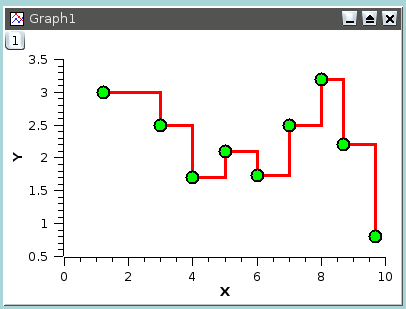
\includegraphics[width=0.4\textwidth,angle=0]{images/beispiel}
%  		\caption{Beispiel Bild; Quelle ist png}
% 		\label{fig:beispiel}
% 		\end{figure}
	
% 	\section{Tabellen}
% 			Lorem ipsum dolor sit amet, consetetur sadipscing elitr, sed diam nonumy eirmod tempor invidunt ut labore et dolore magna aliquyam erat, sed diam voluptua. At vero eos et accusam et justo duo dolores et ea rebum. Stet clita kasd gubergren.

% 		\begin{center}
% 			\begin{tabular}{lcrc} \toprule
% 			Stadium & Substratfreie Kontrolle  & \multicolumn{2}{c}{Probenansatz} \\\cmidrule(rl){3-4}
% 			 & Farbe & Farbe & Bewertung \\\midrule
% 			Alpha1 & farblos & braun & +++ \\
% 			Beta2 & farblos & farblos & - \\\bottomrule 
% 			 \end{tabular}
% 		 \end{center}
		 
% 		2. Beispiel \\
% 		\begin{table}[h]
% 		\centering	 
% 		 	\begin{tabular}{|l|l|c|}
% 			\hline
% 			\textsc{Rang} & \textsc{Name} & \textsc{Rating}\\
% 			\hline
% 			\hline
% 			1 & Garry Kasparov & 2817\\
% 			2 & Viswanathan Anand & 2774\\
% 			3 & Wladimir Kramnik & 2764\\
% 			\hline
% 			\end{tabular}
% 		\caption{Beispiel Beschriftung einer Tabelle}
% 		\label{tab:beispiel}
% 		\end{table}
		
		


% 	\section{Verweise}
% 		Hier werden Verweise auf verschiedene Elemente erstellt.
% 		\subsection{Pageref und Ref} 
% 			Diese Textstelle ist sehr interessant.\label{interessant} \\				
% 			Hier wird auf die Textstelle~\ref{interessant} verwiesen, \\
% 			die sich auf der Seite~\pageref{interessant} befindet.\\[20pt] 
% 			Verweis auf Listing \ref{lst:javaBsp} auf Seite \pageref{lst:javaBsp} \\
% 			Verweis auf Abbildung \ref{fig:beispiel} auf Seite \pageref{fig:beispiel} \\
% 			Verweis auf Tabelle \ref{tab:beispiel} auf Seite \pageref{tab:beispiel}
			
% 	\section{Listing}
% 		\lstset{language=java}
% 		\begin{lstlisting}[frame=hl, caption={Das Listing zeigt Java Quellcode} ,backgroundcolor=\color{gray}, label={lst:javaBsp}]
% /* Java Hallo World Beispiel */

% public class HelloWorld {
%     public static void main(String[] args) {
%         System.out.println("Hello, World");
%     }
% }
% 		\end{lstlisting} 
		
	
\bibliographystyle{plain}
\bibliography{literature}
\pagenumbering{Roman}	
	

	
\end{document}